% !TeX document-id = {296a68f5-c8ec-41d2-ae73-323399fe657a}
% !TeX program = xelatex
% !BIB program = biber
% Compile this file, not individual chapter files.
\documentclass[12pt,a4paper,oneside]{report}

% Compact layout requested for a maximum of three pages for the first subject.
% Deviations from TAMK Guide B: 2 cm left margin and 1.15 line spacing.
% XeLaTeX uses the actual Arial font installed on this computer.
\usepackage{fontspec}
\setmainfont{Arial}
\setsansfont{Arial}
\usepackage[english]{babel}
\usepackage{csquotes}
\usepackage{amsmath}
\usepackage[a4paper,left=2cm,right=2cm,top=2cm,bottom=2cm,
  headheight=15pt,headsep=6mm]{geometry}
\usepackage{setspace}
\setstretch{1.15}
\setlength{\parindent}{0pt}
\setlength{\parskip}{5pt}
\setlength{\emergencystretch}{1em}
\raggedbottom
\clubpenalty=10000
\widowpenalty=10000

\usepackage{graphicx}
\usepackage{xcolor}
\definecolor{tamkpurple}{HTML}{4E008E}
\usepackage{eso-pic}
\usepackage{booktabs}
% Unrelated Java fragment preserved as comments so LaTeX can compile.
% 		if (item.equals("cheese")) {
% 			return new NYStyleCheesePizza();
% 		} else if (item.equals("pepperoni")) {
% 			return new NYStylePepperoniPizza();
% 		} else {
% 			return null;
% 		}
\usepackage{caption}
\captionsetup{font={normalsize,singlespacing},labelfont=normalfont,
  labelsep=period,justification=justified,singlelinecheck=false}
\captionsetup*[table]{position=top}
\captionsetup*[figure]{position=bottom}
\counterwithout{figure}{chapter}
\counterwithout{table}{chapter}

\usepackage{titlesec}
% Compact 12 pt headings, without the report class's large "Chapter" label.
\titleformat{\chapter}[hang]{\normalfont\normalsize\bfseries\raggedright}
  {\thechapter}{1em}{\MakeUppercase}
\titleformat{name=\chapter,numberless}[hang]
  {\normalfont\normalsize\bfseries\raggedright}{}{0pt}{\MakeUppercase}
\titlespacing*{\chapter}{0pt}{-\topskip}{8pt}
\titleformat{\section}{\normalfont\normalsize\bfseries\raggedright}
  {\thesection}{1em}{}
\titleformat{\subsection}{\normalfont\normalsize\bfseries\raggedright}
  {\thesubsection}{1em}{}
\titlespacing*{\section}{0pt}{9pt}{3pt}
\titlespacing*{\subsection}{0pt}{9pt}{3pt}
\AtBeginDocument{%
  \setlength{\abovedisplayskip}{5pt}%
  \setlength{\belowdisplayskip}{5pt}%
  \setlength{\abovedisplayshortskip}{3pt}%
  \setlength{\belowdisplayshortskip}{3pt}%
}
\setlength{\intextsep}{6pt}
\setlength{\textfloatsep}{8pt}
\captionsetup{skip=4pt}
\setcounter{secnumdepth}{2}
\setcounter{tocdepth}{2}
\addto\captionsenglish{\renewcommand{\contentsname}{CONTENTS}}

\usepackage{fancyhdr}
\fancypagestyle{reportpages}{%
  \fancyhf{}%
  \fancyhead[R]{\normalfont\normalsize\thepage}%
  \renewcommand{\headrulewidth}{0pt}%
  \renewcommand{\footrulewidth}{0pt}%
}
\fancypagestyle{plain}{%
  \fancyhf{}%
  \fancyhead[R]{\normalfont\normalsize\thepage}%
  \renewcommand{\headrulewidth}{0pt}%
  \renewcommand{\footrulewidth}{0pt}%
}

% APA 7 baseline. Check source-specific TAMK adaptations when adding entries.
\usepackage[backend=biber,style=apa]{biblatex}
\DeclareLanguageMapping{english}{english-apa}
\AtBeginBibliography{\singlespacing\raggedright}
\setlength{\bibitemsep}{\baselineskip}
\usepackage{xurl}
\usepackage[hidelinks,unicode]{hyperref}
\urlstyle{same}

% Edit the title-page information here.
\newcommand{\ReportTitle}{Modern AI Systems}
\newcommand{\ReportSubtitle}{From Local LLMs to Software Engineering Agents}
\newcommand{\ReportAuthor}{Daniel Tempel}
\newcommand{\ReportType}{COURSE REPORT}
\newcommand{\ReportDate}{October 2026}
\newcommand{\ReportCourse}{5G00GC12-3001}
% Optional: fill in the degree programme when its exact name is known.
\newcommand{\ReportProgramme}{}

\hypersetup{pdftitle={\ReportTitle},pdfauthor={\ReportAuthor},
  pdfsubject={\ReportSubtitle},pdflang={en-GB}}

\addbibresource{references.bib}

\begin{document}
% Preserve the template cover while the report body uses compact margins.
\newgeometry{left=4cm,right=2cm,top=2cm,bottom=2cm}
\begin{titlepage}
\thispagestyle{empty}
% Original cover artwork extracted from the user-supplied Word template.
\AddToShipoutPictureBG*{%
  \AtPageLowerLeft{
\includegraphics[width=\paperwidth,height=\paperheight]{assets/tamk-cover.png}}%
}
\begingroup
\setlength{\parskip}{0pt}
\setstretch{1}
% The title sits below the large pale emblem, as in the Word template.
\vspace*{14.7cm}
{\color{tamkpurple}\fontsize{26}{31}\selectfont\bfseries
  \raggedright\ReportTitle\par}
\vspace{0.35cm}
{\color{tamkpurple}\fontsize{16}{20}\selectfont
  \raggedright\ReportSubtitle\par}
\vspace{0.9cm}
{\fontsize{14}{18}\selectfont\ReportAuthor\par}
\vfill
{\fontsize{12}{15}\selectfont
  \ReportType\par
  \ReportDate\par
  \vspace{0.45cm}
  \ReportCourse\par
  \ReportProgramme\par}
\endgroup
\end{titlepage}
\restoregeometry

% The cover counts as page 1 but has no visible page number.
\setcounter{page}{2}
\pagestyle{reportpages}
% !TeX root = ../Tempel-Daniel.tex
\chapter*{PREFACE}
\addcontentsline{toc}{chapter}{PREFACE}

Artificial intelligence is becoming an increasingly important field in software engineering, and I see it as a promising direction for my future career. I am particularly interested in developing AI agents that can perform practical tasks and be integrated into production software systems.

My main motivation for this report was to understand how such systems can be built using both locally deployed language models and powerful models accessed through external APIs. I believe that understanding these technologies, their architectural requirements and their practical limitations will become an increasingly valuable skill for software developers.

For this reason, I decided to organise the selected topics as a technical walkthrough, starting with the fundamentals of language models and gradually progressing towards tool integration, context management, autonomous agents and production architecture.

The report follows this progression using an AI Software Engineering Assistant as a recurring example. My goal was to develop a structured understanding of the technologies involved and how they can work together in real-world software applications.

Generative AI tools were used to support topic exploration, source discovery, drafting and language revision during the preparation of this report. All technical claims, references and final content were critically reviewed and verified by the author.

\begingroup
% Keep the growing contents compact without changing body text.
\small
\singlespacing
\setlength{\parskip}{0pt}
\makeatletter
\patchcmd{\l@chapter}{\vskip 1.0em \@plus\p@}{\vskip 0.4em \@plus\p@}{}{\PackageError{report-layout}{Could not compact chapter spacing in contents}{Check the report class definition of l@chapter.}}
\makeatother
\tableofcontents
\endgroup

% !TeX root = ../Tempel-Daniel.tex
\chapter{Introduction}
\label{chap:introduction}

Large language models (LLMs) are increasingly used as components of software development tools. Modern AI-assisted development systems can analyse source code, explain errors, generate modifications and interact with external tools such as version-control systems, test runners and documentation sources. However, building such a system requires more than selecting a capable language model. Model deployment, context management, tool integration, retrieval, security and evaluation all influence whether the resulting system is practical and reliable.

This report examines these topics through a common example: an \textbf{AI Software Engineering Assistant} whose task is to analyse a GitHub issue, inspect the relevant source code, propose a modification and verify the solution by running tests. The same use case is developed throughout the report so that the individual AI concepts can be considered as parts of one system rather than as isolated technologies.

The report begins with the foundations of running large language models locally and the hardware constraints this creates. It then considers how models can be compared and selected for a software-engineering workload. Later sections extend the assistant with structured outputs and tool use, context management, retrieval, the Model Context Protocol and autonomous agent behaviour. Finally, production architecture, security and evaluation are considered to examine how such a system could be operated reliably.

The aim is not to implement a complete production assistant, but to understand the main architectural concepts and trade-offs involved in constructing modern AI systems for software engineering.

% !TeX root = ../Tempel-Daniel.tex
% Mandatory subject 1: Understanding Local LLM Models.
\chapter{Understanding Local LLM Models}
\label{chap:local-llms}

% Keep the expanded chapter compact without changing body font or line spacing.
\begingroup
\setlength{\parskip}{3pt}
\setlength{\abovedisplayskip}{3pt}
\setlength{\belowdisplayskip}{3pt}

Local inference means that the model weights and the computations required to generate responses are located on hardware controlled by the user rather than being accessed through a remote inference API. For a software-engineering system, this can provide greater control over deployment and reduce the need to transmit project source code to an external service.

The main limitation is hardware capacity. Model weights must be accommodated within the available system and GPU memory, while context processing and intermediate computations require additional runtime memory. Understanding parameters, numerical representation and context memory is therefore necessary before deciding which models are technically practical for local execution.

\section{From source code to model output}

Input text is processed by a tokenizer, which converts it into tokens and numerical token IDs. These are transformed into vector representations and processed through Transformer layers. Transformer layers combine attention mechanisms and feed-forward networks containing large learned weight matrices \parencite{vaswani2017attention}.

Figure~\ref{fig:local-inference-pipeline} traces the conversion of repository input into a generated token and its return to the context for the next generation step.

\begin{figure}[htbp]
\centering
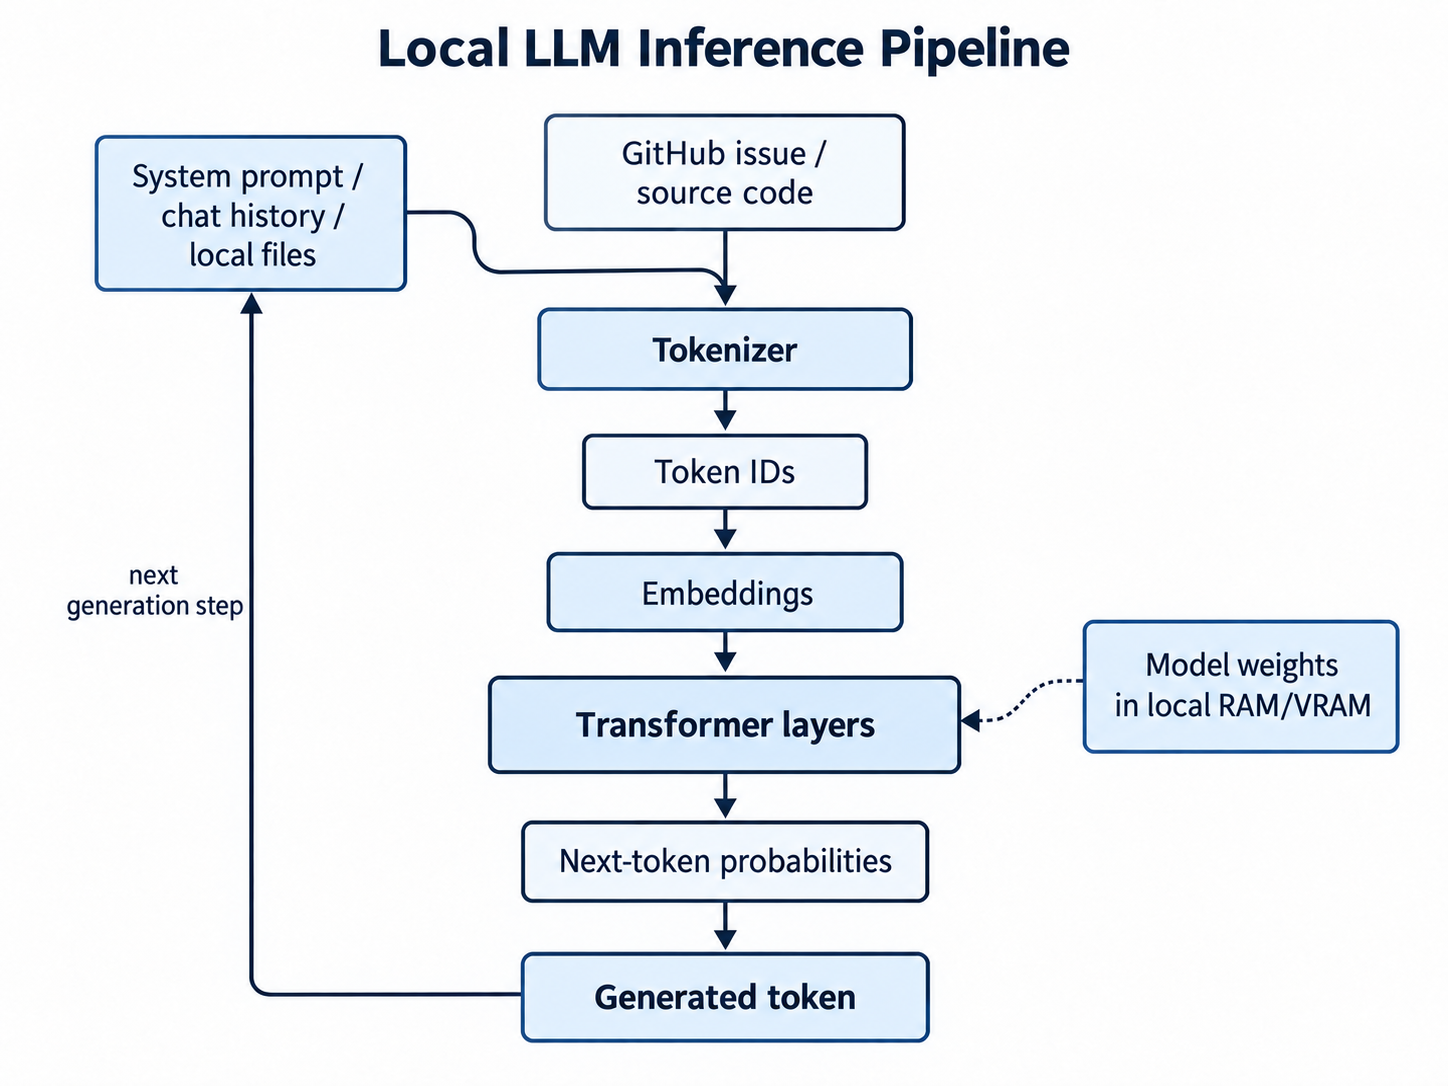
\includegraphics[width=11.5cm]{images/local-llm-inference-pipeline-autoregressive.png}
\caption{Simplified local LLM inference pipeline.}
\label{fig:local-inference-pipeline}
\end{figure}

The feedback path represents autoregressive generation: each predicted token becomes part of the context for the following step.

A model described as 8B contains approximately eight billion learned parameters, most of which are weights. These weights do not individually represent specific facts or concepts; learned information is distributed across large collections of parameters.

The number of parameters alone does not determine the memory required to store the model weights. Their numerical representation is equally important.

\section{Precision and quantization}

A useful approximation of model weight memory is
\[
M_{\text{weights}}
\approx
\frac{N_{\text{parameters}}\times b}{8},
\]
where \(b\) is the number of bits used per parameter.

FP16 uses 16 bits, or two bytes, per value. An idealised 8B model therefore requires approximately
\[
8\times 10^9 \times 2
\approx
16\text{ GB}
\]
for its weights. This calculation uses decimal gigabytes, while the model sizes in Figure~\ref{fig:llama-quantization} are reported in binary gibibytes (GiB).

Quantization reduces memory requirements by representing weights with fewer bits. In a simplified symmetric scheme,
\[
q=\operatorname{round}(w/s),
\]
where \(w\) is the original weight, \(s\) is a scale and \(q\) is a low-bit integer representation. The approximate value can later be reconstructed as
\[
\hat{w}=sq.
\]
For example, with \(s=0.1\), a weight of \(0.27\) can be stored as \(q=3\), which reconstructs to \(0.30\). This introduces quantization error. In practice, scales are typically shared by blocks of weights.

A theoretical 4-bit representation of an 8B model would require about 4 GB. Real quantization schemes also use scaling information, metadata and, in some cases, different representations for different tensors. Therefore, a scheme labelled Q4 does not imply exactly four bits per weight.

% Keep the bar chart next to its interpretation.
\noindent\begin{minipage}{\linewidth}
\centering
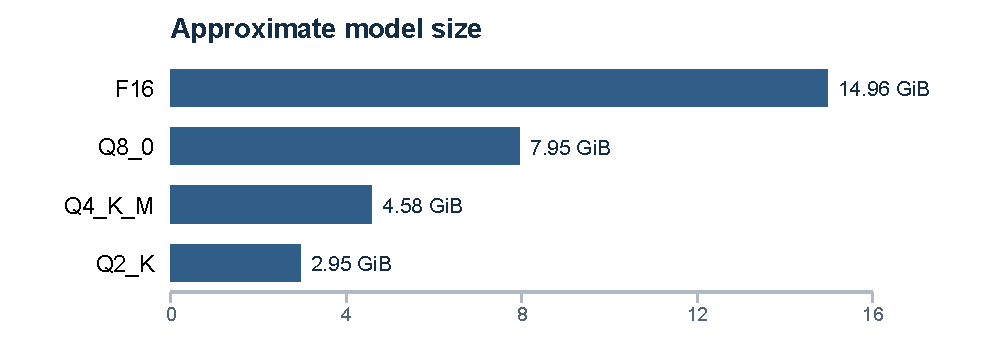
\includegraphics[width=14cm]{images/model-size-comparison.pdf}
\captionsetup{hypcap=false}
\captionof{figure}{Approximate model file sizes for different representations of Llama 3.1 8B, based on llama.cpp data \parencite{ggml-quantize}.}
\label{fig:llama-quantization}
\end{minipage}

The chart shows why quantization is useful for local deployment. \texttt{Q4\_K\_M} reduces the model file size from about 15 GiB to less than 5 GiB. The relationship between bit width and task quality is not linear: the effect depends on the model, quantization scheme and target task \parencite{ggml-quantize}.

Quantization can also improve inference speed because smaller weights reduce memory traffic. However, lower bit width does not automatically produce proportional speedups, since performance also depends on hardware support, kernels and quantization overhead.

GGUF, \texttt{Q4\_K\_M} and \texttt{llama.cpp} describe different layers of the system. GGUF is a model file format, \texttt{Q4\_K\_M} is a model quantization scheme that can use a mixture of tensor representations, and \texttt{llama.cpp} is an inference runtime that can load and execute such models \parencite{ggml-quantize,ggml-models}.

Low-precision model formats are not all equivalent. FP8 remains a floating-point representation rather than an integer-style block quantization format. Common FP8 variants include \texttt{E4M3} and \texttt{E5M2}, which trade numerical precision against dynamic range \parencite{nvidia-fp8}. Whether FP8 improves inference performance depends strongly on hardware and runtime support.

GGUF quantization names encode different quantization recipes rather than a uniform number of bits for every tensor. Common llama.cpp variants span low-bit families such as \texttt{Q2\_K}, \texttt{Q3\_K\_M}, \texttt{Q4\_K\_M}, \texttt{Q5\_K\_M} and \texttt{Q6\_K} up to \texttt{Q8\_0}. The leading number indicates the approximate precision class, while the actual effective bits per weight can differ because scales, metadata and mixed tensor representations add overhead. The K suffix identifies the K-quant family, while suffixes such as S and M distinguish smaller and medium mixed-precision variants. IQ variants, such as \texttt{IQ2\_XS} or \texttt{IQ3\_M}, use importance-aware low-bit quantization approaches. Prefixes such as UD are publisher-specific rather than core llama.cpp quantization types; Unsloth uses them for its Dynamic GGUF variants, where quantization choices may differ between layers to preserve quality \parencite{ggml-quantize,unsloth-dynamic}.

An alternative direction is to design models for extremely low-bit weights from the beginning rather than quantizing an already trained high-precision model. BitNet b1.58, for example, uses ternary weights \(\{-1,0,+1\}\), corresponding conceptually to about \(\log_2(3)\approx1.58\) bits of information per weight \parencite{ma2024bitnet}. This is a different model-design approach rather than simply another Q4-like format. Native low-bit designs can substantially reduce model-weight storage and memory-bandwidth requirements compared with conventional FP16 models. This can change the hardware cost of inference when suitable kernels and hardware support are available, although the theoretical reduction in bit width does not automatically translate into an equivalent end-to-end speedup.

\section{Runtime memory and context}

Model file size is not equal to runtime memory. A simplified model is
\[
M_{\text{runtime}}
\approx
M_{\text{weights}}
+
M_{\text{KV cache}}
+
M_{\text{temporary}}
+
M_{\text{runtime overhead}}.
\]
Therefore, a 4.6 GiB model file does not imply that 4.6 GiB of VRAM is sufficient.

For the assistant, the active context may include system instructions, a GitHub issue, repository structure, source files, previous messages, tool results and the response generated so far.

Three different context-related limits should be distinguished: the maximum context length supported by the model, the context size configured by the inference runtime, and the number of tokens actually used by a particular request. The amount of allocated KV-cache memory also depends on runtime configuration. Dynamic caches grow as more tokens are processed, while static caches may reserve capacity for a configured maximum in advance \parencite{hf-cache-strategies}.

Inference can be divided into two stages. During \textbf{prefill}, the model processes the existing context. During \textbf{decode}, it generates new tokens one by one. Transformer self-attention produces Query, Key and Value representations. Previously calculated Key and Value vectors can be stored in a \textbf{KV cache}, avoiding repeated computation during generation \parencite{hf-cache-strategies}.

The trade-off is additional memory consumption. With a dynamic cache, longer prompts, generated output and tool results appended to subsequent model requests increase the amount of active context. This is especially relevant for the assistant, which may process large source files or long test logs.

% Crop only the outer whitespace and embedded "Figure 2" caption in LaTeX.
% The original PNG is preserved unchanged; keep the diagram before its discussion.
Figure~\ref{fig:local-runtime-memory} separates model weights from the additional memory required for context and execution, explaining why model file size alone is insufficient for capacity planning.

\noindent\begin{minipage}{\linewidth}
\centering
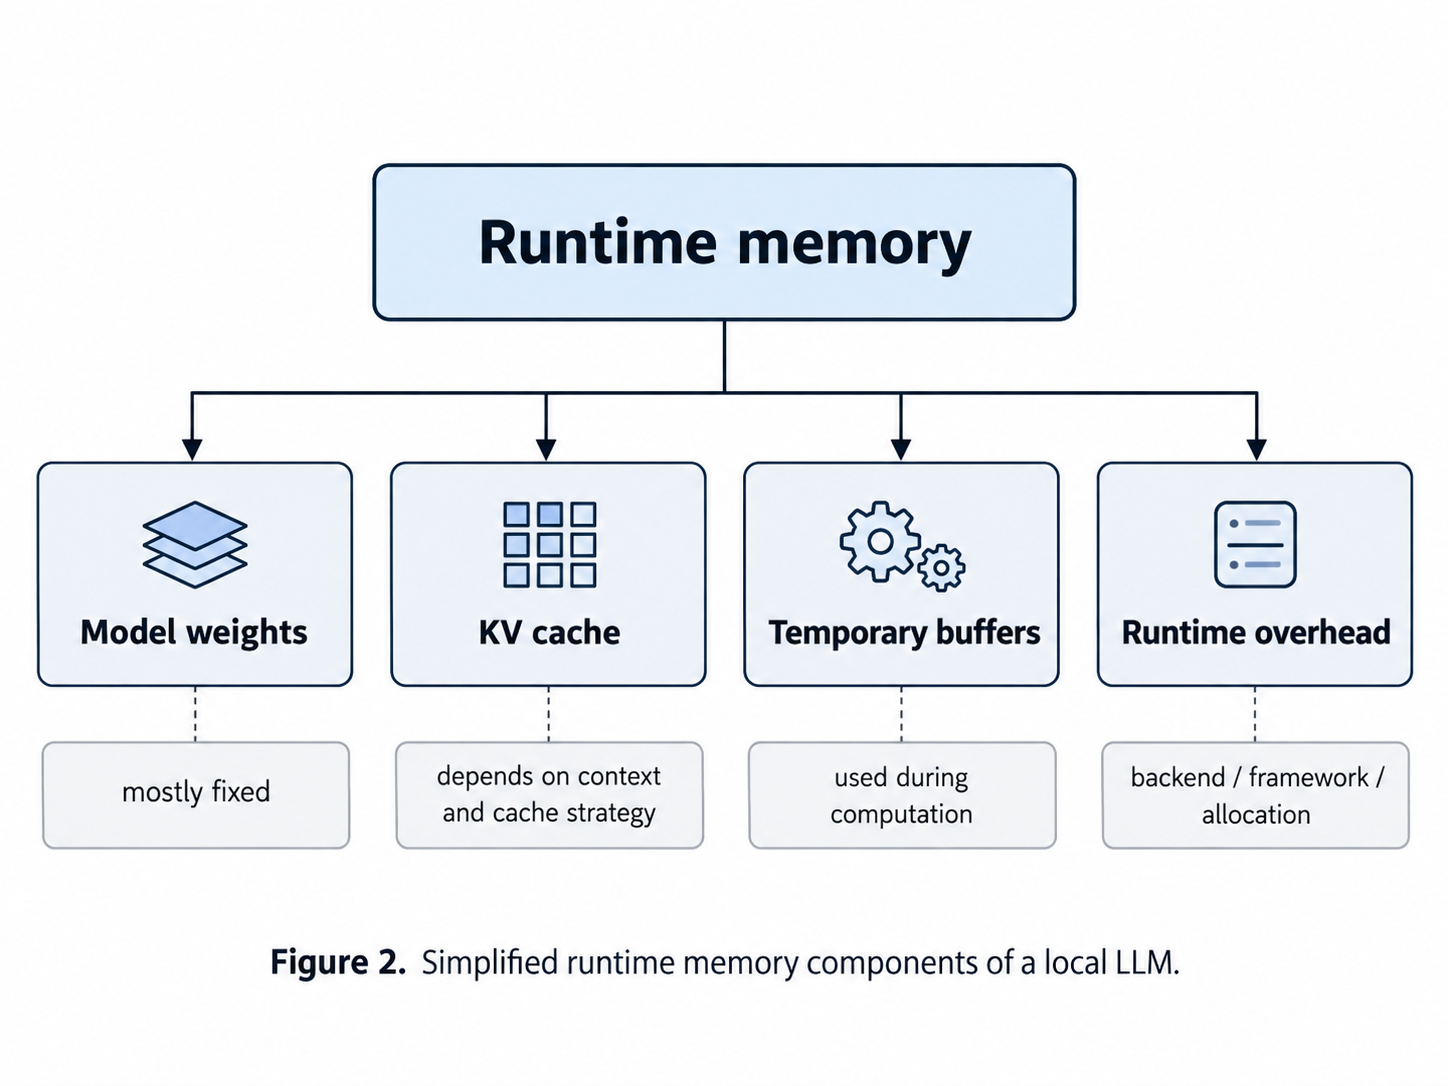
\includegraphics[width=13cm,trim=0 165bp 0 125bp,clip]{images/local-llm-runtime-memory.png}
\captionsetup{hypcap=false}
\captionof{figure}{Simplified runtime memory components of a local LLM.}
\label{fig:local-runtime-memory}
\end{minipage}

Attention architecture also affects KV-cache size. Multi-Head Attention uses many separate Key/Value heads, Multi-Query Attention uses one shared Key/Value head, and Grouped-Query Attention uses an intermediate number. Reducing the number of KV heads can lower context-memory requirements \parencite{ainslie2023gqa}.

\section{Model specialisation and deployment trade-offs}

Model specialisation is independent of quantization and local execution. A general-purpose model targets broad language tasks, while specialised models can focus on domains such as programming. Separately, instruction-tuned models are post-trained to follow user instructions effectively. A model can therefore be coding-specialised, instruction-tuned, quantized and executed locally at the same time.

For the assistant, the largest available model is not automatically the most practical choice. A smaller coding-specialised, instruction-tuned model that fits comfortably into GPU memory may be more practical to deploy than a much larger general-purpose model that requires aggressive quantization or CPU offloading.

However, practical suitability cannot be determined from parameter count or memory usage alone. Candidate models should therefore be evaluated not only on coding benchmarks, but also on their ability to follow tool-use instructions and produce changes that pass relevant tests, while remaining within the available memory, context and latency budget. These evaluation criteria lead directly to the next topic: \textbf{LLM Benchmarks and Model Selection}.

% Finish this chapter before restoring the document spacing.
\par\clearpage
\endgroup

% !TeX root = ../Tempel-Daniel.tex
\chapter{LLM Benchmarks and Model Selection}
\label{chap:benchmarks}

Chapter~\ref{chap:local-llms} explained how model size, numerical representation and context requirements constrain local LLM deployment. These constraints determine which configurations are technically feasible, but not whether they can reliably perform the intended software-engineering tasks. Published benchmark results provide useful evidence, but only under particular tasks and evaluation conditions.

A benchmark is a standardised collection of tasks with a scoring procedure, whereas evaluation also includes the prompt, context, tools, execution limits and success criteria. Model selection uses this evidence to identify suitable candidates for a specific application. Frameworks such as HELM therefore evaluate language models across multiple scenarios and metrics rather than reducing capability to a single score \parencite{liang2022helm}.

In a practical deployment, candidate models should be compared within a fixed assistant architecture. Such results would describe their suitability for the target application rather than model capability in isolation. Candidates should also be treated as concrete deployment configurations, including the model version, quantization scheme, inference runtime, and runtime configuration intended for deployment.

\section{Evaluating software engineering capabilities}
\label{sec:engineering-capabilities}

Different benchmarks measure different capabilities, and their relevance depends on the target workload. General-purpose benchmarks such as MMLU-Pro evaluate knowledge and reasoning across multiple domains. MMLU-Pro was designed as a more difficult and less prompt-sensitive successor to MMLU, while Humanity's Last Exam was motivated partly by the increasing saturation of established academic benchmarks \parencite{wang2024mmlupro,phan2025hle}. Such evaluations provide evidence about broad reasoning ability but do not directly measure repository-level software engineering.

Coding benchmarks move closer to the intended workload. LiveCodeBench continuously incorporates recently published programming problems and evaluates capabilities including code generation, execution and self-repair \parencite{jain2024livecodebench}. Using recently published tasks can reduce contamination risk relative to static datasets, although their publication dates must still be considered in relation to the training cutoff of the evaluated model. Execution-based evaluation is particularly useful for programming because different implementations can be textually different while exhibiting the same correct behaviour.

Repository-level work introduces additional requirements such as code navigation, integration with existing components and regression control. SWE-Lancer contains more than 1,400 tasks originating from real freelance software-engineering work. Its independent engineering tasks are evaluated using end-to-end tests, while a separate category of managerial tasks requires choosing between technical implementation proposals \parencite{miserendino2025swelancer}.

Tool-based environment interaction represents another relevant evaluation dimension. Terminal-Bench 2.0 evaluates systems in command-line environments where they must inspect the environment, execute commands, observe results and complete multi-step tasks \parencite{merrill2026terminalbench}. This becomes relevant when an LLM is embedded into an interactive system rather than used only for single-response generation.

Figure~\ref{fig:evaluation-dimensions} relates these complementary benchmark dimensions to the representative assistant tasks that a deployment evaluation should cover.

\noindent\begin{minipage}{\linewidth}
\centering
% Trim only outer whitespace; preserve all labels and the explanatory footer.
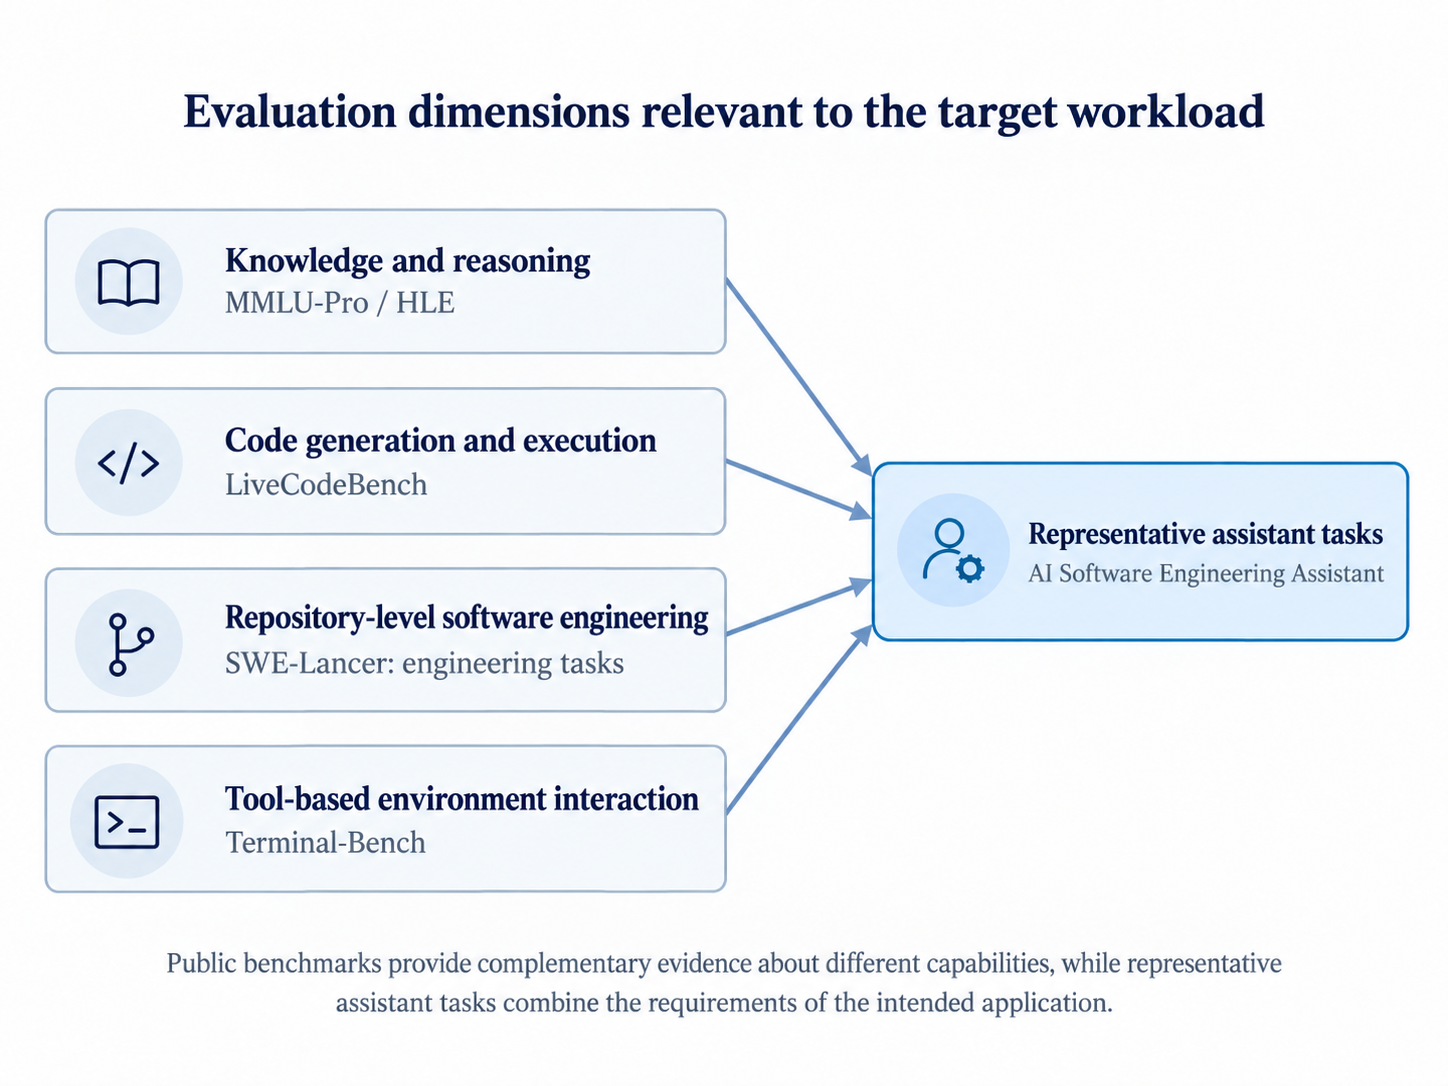
\includegraphics[width=14cm,trim=0 45bp 0 60bp,clip]{images/benchmark-evaluation-dimensions.png}
\captionsetup{hypcap=false}
\captionof{figure}{Evaluation dimensions relevant to the target workload of the AI Software Engineering Assistant. The dimensions overlap; the listed benchmarks are illustrative examples.}
\label{fig:evaluation-dimensions}
\end{minipage}

Figure~\ref{fig:evaluation-factors} shows why measured performance depends on the assistant configuration and execution conditions as well as the model. The evaluation harness initialises the task environment, executes the assistant under defined limits and records the resulting actions and outputs. The evaluator and acceptance tests then determine whether the resulting solution satisfies the task requirements.

\noindent\begin{minipage}{\linewidth}
\centering
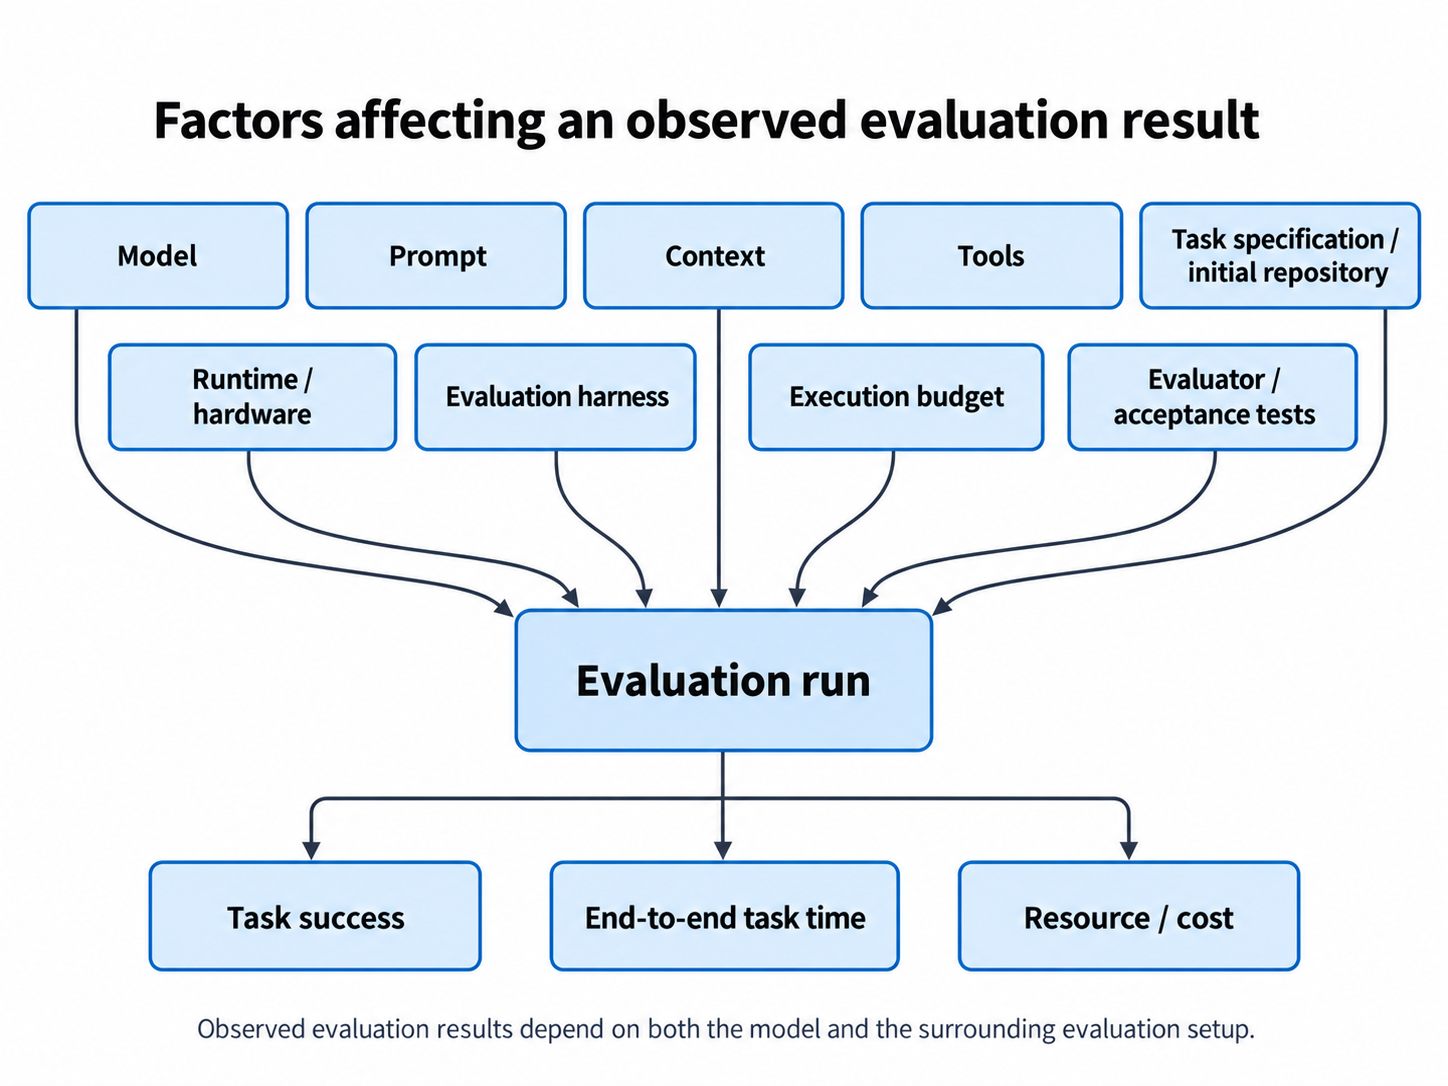
\includegraphics[width=14cm,trim=0 45bp 0 60bp,clip]{images/evaluation-result-factors.png}
\captionsetup{hypcap=false}
\captionof{figure}{Factors influencing an observed evaluation result, including the assistant configuration, task conditions, execution environment and independent verification.}
\label{fig:evaluation-factors}
\end{minipage}

Candidate models should therefore be compared under controlled conditions. Each candidate should receive the same task specification, initial repository state, system prompt, context policy, tools and execution budget. One evaluation run may contain several internal actions, such as editing code, running tests and revising a failed solution. A repeated run instead restarts the task from the same initial state. Providing one candidate with additional runs or a larger execution budget would make the results less comparable.

\section{Reliability and limitations of LLM evaluation}
\label{sec:evaluation-limitations}

Benchmark scores remain imperfect measurements. Saturation reduces their ability to distinguish advanced models, while data contamination can occur when public benchmark tasks later appear in training corpora. Evaluation results may also vary between runs because LLM generation can be stochastic. Small differences should therefore be interpreted cautiously, and the number of evaluated tasks and repeated runs should be reported where relevant.

Tasks used to tune prompts, context strategies or other parts of the assistant should also be separated from those used for final comparison. Otherwise, the system may become indirectly optimised for its own evaluation set.

A further limitation is evaluator validity. Execution-based evaluation is stronger than judging whether generated code merely appears plausible, but passing tests is meaningful only when the specification and tests correctly represent the intended behaviour. A 2026 audit of the 731-task public SWE-Bench Pro split illustrates this problem. After an automated filter identified potentially problematic tasks, OpenAI reported breaking evaluation issues in 200 tasks through a human-supervised agent audit and in 249 tasks through human annotation, corresponding to 27.4\% and 34.1\% of the full public split \parencite{openai2026codingaudit}. Reported problems included underspecified requirements, tests enforcing unstated implementation details, insufficient test coverage and conflicts between task descriptions and evaluators.

Such problems can produce errors in both directions: a valid implementation may fail because an evaluator checks an unstated requirement, while an incomplete implementation may pass because relevant behaviour is not covered. Execution-based evaluation is therefore only as reliable as its task specification and test suite.

The same principle should apply to an internal evaluation of the assistant. Task descriptions and acceptance criteria should be reviewed before comparison, and final verification should use fixed evaluation tests that the assistant cannot modify. Ambiguous outcomes should be checked against predefined acceptance criteria.

\section{Model selection for the assistant}
\label{sec:assistant-model-selection}

Public benchmarks should primarily be used to create a shortlist. Deployment constraints from Chapter~\ref{chap:local-llms} can first exclude configurations that do not satisfy hardware or runtime requirements. Relevant reasoning, coding and software-engineering benchmarks can then provide preliminary evidence about the remaining candidates.

The final comparison should use representative repository-level tasks, such as bug fixing, API changes, database validation, refactoring and coordinated multi-file modifications. Candidate configurations should be evaluated under the same task, environment and execution conditions defined in Section~\ref{sec:engineering-capabilities}.

Task success should be the primary quality metric. A successful task should require the requested behaviour to be implemented, predefined acceptance tests to pass and existing regression tests to remain successful. Results should also be examined by task category, since two candidates with similar overall success rates may fail on different types of work.

Operational metrics provide additional information once candidates satisfy the required quality level. End-to-end task time is more relevant than time to first token for workflows involving repository inspection, multiple model calls and repeated test execution. Completion time should be interpreted together with task success, with failed runs and timeouts reported separately. Resource measurements should cover the complete evaluation run, including model inference and tool execution. For API-hosted models this may include token or request cost, while local configurations can instead be compared using hardware utilisation, execution time or an explicitly defined compute cost. Any cost-per-success metric should also include resources consumed by failed runs.

Model selection should therefore follow predefined requirements rather than simply choosing the highest benchmark score. Candidates that fail the required quality or deployment constraints should be excluded; the remaining configurations can then be compared using task success, completion time and resource consumption.

This chapter defines the criteria and procedure for a preliminary model shortlist rather than selecting a final model in isolation. Final selection requires testing the remaining candidates within the assistant's actual tool, context and interaction architecture, which is developed in the following chapters.

% !TeX root = ../Tempel-Daniel.tex
\chapter{Structured Outputs, Function Calling and Tool Use}
\label{chap:tool-use}


The previous chapter described how candidate models can be evaluated within the intended software-engineering workload. However, selecting a capable model is not sufficient to build the AI Software Engineering Assistant. A language model can generate explanations, code and recommendations, but free-form text alone does not provide a reliable software interface to repositories, test runners, databases or external APIs. The assistant therefore requires mechanisms that turn model generation into machine-readable data and action requests that conventional software components can process.

As described in Chapter~\ref{chap:local-llms}, an LLM still generates tokens autoregressively. Structured output and function calling do not change this basic inference process or give the model direct access to external systems. Instead, they constrain and interpret parts of the generated output so that the model can interact with the surrounding application through defined interfaces.

\section{Structured outputs as a machine-readable interface}
\label{sec:structured-outputs}

A free-form response may express the intended information correctly while still being difficult for software to process reliably. For example, a model could identify \texttt{src/auth.py} as the affected file using many different natural-language formulations. Returning the same information as structured data creates a more explicit interface:

\noindent\begin{minipage}{\linewidth}
\small\singlespacing
\begin{verbatim}
{
  "affected_file": "src/auth.py",
  "needs_fix": true
}
\end{verbatim}
\end{minipage}

JSON provides a machine-readable representation, but syntactically valid JSON alone does not guarantee that an application receives the expected fields and data types. JSON Schema provides a formal vocabulary for describing the structure and validation constraints of JSON documents \parencite{jsonschema2022}. A schema can, for example, require \texttt{affected\_file} to be a string and \texttt{needs\_fix} to be a Boolean.

This distinction also appears in current LLM APIs. JSON mode constrains a response to valid JSON, whereas schema-constrained output additionally constrains its structure to a supplied schema. OpenAI refers to the latter capability as \emph{Structured Outputs} and explicitly distinguishes it from JSON mode \parencite{openai-structured-outputs}.

Schema constraints can be applied during generation rather than only after a complete response has been produced. An inference runtime can restrict candidate output according to a grammar derived from the required structure. The llama.cpp inference runtime introduced in Chapter~\ref{chap:local-llms}, for example, supports GBNF grammars and can convert a supported subset of JSON Schema into such grammars \parencite{ggml-grammars}.

Constraining the output format does not, however, replace instructions describing the intended meaning of its fields. In llama.cpp, a JSON schema used for ordinary constrained output is not automatically visible to the model and must be complemented by an appropriate prompt; tool-calling schemas are handled differently and are supplied as part of the model interaction \parencite{ggml-grammars}.

Structural correctness must therefore be separated from semantic correctness. An argument such as \texttt{"path": "banana.py"} may satisfy a schema requiring a string while still referring to a file that does not exist in the selected repository. Likewise, a schema cannot determine whether inspecting that file is the appropriate action for the current task. Schema-constrained output improves the reliability of the interface, but it does not establish the correctness of the generated values or decisions.

Schema adherence is also separate from successful request completion. A response may remain incomplete because of output limits or inference/API failures, while a refusal may be returned instead of the requested structure. Providers and inference runtimes may additionally support only subsets of the full JSON Schema language. Applications must therefore distinguish request completion, structural validity and semantic validity.

\section{Function calling and tool execution}
\label{sec:function-calling}

Structured output is useful when an application requires structured information. Function calling applies a similar interface to actions. Instead of returning only data, the model can generate a structured request identifying an available operation and the arguments required to invoke it. A request to inspect a source file could conceptually be represented as:

\noindent\begin{minipage}{\linewidth}
\small\singlespacing
\begin{verbatim}
{
  "name": "read_file",
  "arguments": {
    "path": "src/auth.py"
  }
}
\end{verbatim}
\end{minipage}

The corresponding tool definition usually contains a name, description and schema for its arguments. The model therefore receives a description of an available capability rather than the implementation of the underlying function.

Function calling does not by itself guarantee that generated arguments satisfy the declared schema. This depends on the API or inference runtime and the constraint mode being used. OpenAI, for example, distinguishes strict function calling, which enforces the supplied function schema through Structured Outputs, from non-strict best-effort generation \parencite{openai-function-calling}.

The execution boundary is central to the assistant architecture. The LLM does not itself open files, execute tests or call remote APIs. It generates a structured request for an operation. The assistant runtime receives this request, validates its arguments, checks that the requested operation is permitted within the task's allowed scope and dispatches the corresponding software operation. The result is then returned to the runtime and can be included in a subsequent model request.

\noindent\begin{minipage}{\linewidth}
\centering
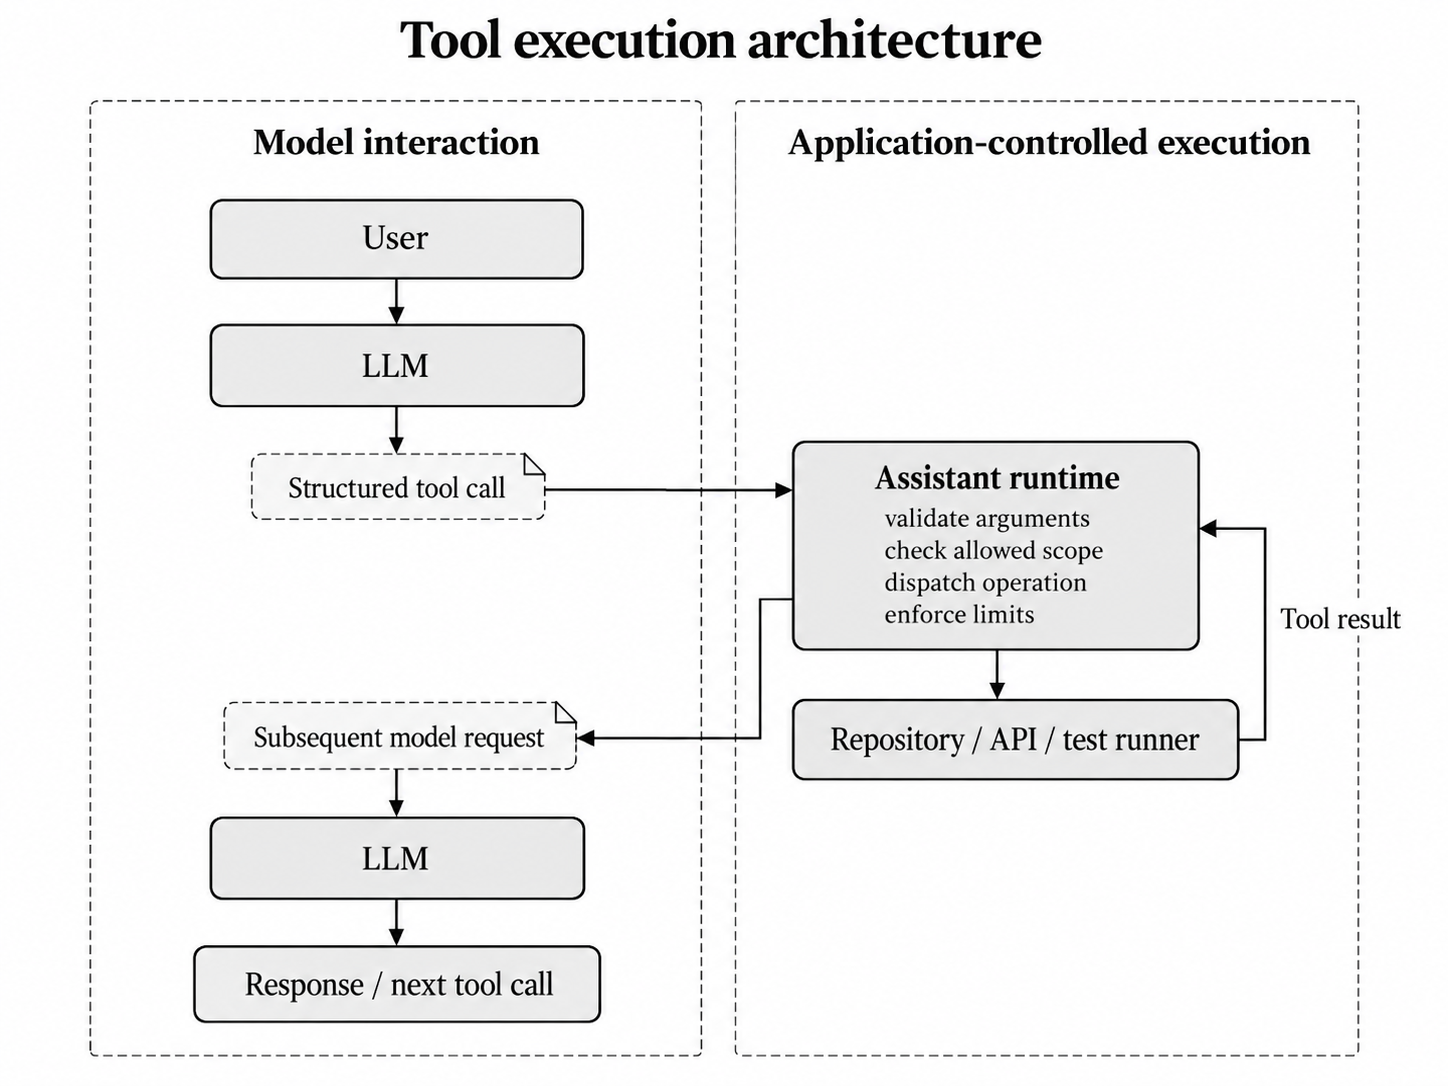
\includegraphics[width=15cm]{images/tool-execution-architecture.png}
\captionsetup{hypcap=false}
\captionof{figure}{Separation between model-generated tool requests and application-controlled tool execution in the AI Software Engineering Assistant.}
\label{fig:tool-execution}
\end{minipage}


This interaction can be summarised as:

\begin{center}
\small\singlespacing
\begin{tabular}{c}
User \\
\(\downarrow\) \\
LLM \\
\(\downarrow\) structured tool call \\
Assistant runtime \\
\(\downarrow\) \\
Repository / API / test runner \\
\(\downarrow\) tool result \\
Assistant runtime \\
\(\downarrow\) subsequent model request \\
LLM \\
\(\downarrow\) \\
response or subsequent tool call \\
\end{tabular}
\end{center}

The execution environment does not necessarily have to be the developer's own process. Some platforms provide tools executed by provider infrastructure, while others return tool requests to the client application for execution. The architectural distinction remains the same: generation specifies an operation, while the actual operation is performed outside the model itself.

Tool results provide new observations that can be included in the model's active context. If \texttt{read\_file} returns the current contents of \texttt{src/auth.py}, the model can reason over that repository state rather than relying on information encoded in its weights. Tool use therefore connects model reasoning to current external state while preserving a software-controlled execution boundary.

\section{Tool interaction and practical constraints}
\label{sec:tool-constraints}

The interaction can be illustrated using the recurring task \emph{Fix GitHub issue \#42 and verify the solution}. The assistant could first request \texttt{get\_issue(42)} to retrieve the current issue description. If the issue refers to missing handling of an \texttt{Authorization} header, the model could then request \texttt{search\_code("Authorization")} followed by \texttt{read\_file("src/auth.py")}. After identifying the required modification, it could request an \texttt{apply\_patch} operation to change the repository and then invoke \texttt{run\_tests(...)} to evaluate the modified state.

This sequence separates generation of a proposed change from its application to the repository. Producing corrected source code does not itself modify a file; the modification occurs only when the corresponding tool operation is executed by the surrounding system.

At each interaction step, several different forms of correctness should be distinguished:

\noindent\begin{minipage}{\linewidth}
\captionsetup{hypcap=false}
\captionof{table}{Levels of correctness in model-generated tool requests.}
\label{tab:tool-failures}
\small\singlespacing
\renewcommand{\arraystretch}{1.15}
\begin{tabular}{@{}p{2.0cm}p{6.5cm}p{7.0cm}@{}}
\toprule
{\raggedright\textbf{Failure level}\par} & \textbf{Question} & \textbf{Example} \\
\midrule
{\raggedright Syntax\par} & {\raggedright Can the generated request be parsed?\par} & {\raggedright Malformed JSON\par} \\
{\raggedright Schema\par} & {\raggedright Does it satisfy the declared tool contract?\par} & {\raggedright Missing required \texttt{path}\par} \\
{\raggedright Semantic\par} & {\raggedright Do the arguments satisfy the operation's preconditions in the current environment?\par} & {\raggedright Requesting a file that does not exist in the selected repository\par} \\
{\raggedright Decision\par} & {\raggedright Is the requested operation appropriate for the task?\par} & {\raggedright Requesting a file modification when the user asked for read-only analysis\par} \\
\bottomrule
\end{tabular}
\end{minipage}

Strict schema-constrained generation can substantially reduce syntax and schema failures, but it cannot establish semantic validity or the quality of the model's action selection. Those properties depend on the current environment, task requirements and model reasoning.

Tool execution can also fail independently of the generated request. A file may have been removed, an external API may return an error or a test process may exceed its execution limit. Rather than hiding such failures, the assistant runtime can return them as structured tool results:

\noindent\begin{minipage}{\linewidth}
\small\singlespacing
\begin{verbatim}
{
  "ok": false,
  "error": "FILE_NOT_FOUND",
  "path": "src/auth.py"
}
\end{verbatim}
\end{minipage}

Such a result can be added to the next model request, allowing the model to revise its next action. Repeated model–tool interaction therefore creates a feedback loop between model-generated decisions and observations obtained through actual tool execution. The runtime can additionally enforce execution limits and determine whether another interaction step is permitted or control should return to the user.

\begingroup
\setlength{\emergencystretch}{2em}
Tool interaction also introduces operational overhead. Tool definitions and argument schemas must be made available to the model, while generated calls and returned results increase the amount of information exchanged across model requests. Multiple model–tool rounds add execution latency, and returned results may increase the active context described in Chapter~\ref{chap:local-llms}.
\par\endgroup

Function calling and tool execution therefore provide the interface through which the AI Software Engineering Assistant can interact with external software, but they do not determine which repository information, previous observations or available capabilities should be presented to the model at a particular step. As the available information grows, selecting and maintaining the relevant active context becomes a separate architectural problem. This is addressed in the following chapter on Context Engineering and Memory.

% !TeX root = ../Tempel-Daniel.tex
\chapter{Context Engineering and Memory}
\label{chap:context-memory}

The previous chapter showed how structured tool calls allow the AI Software Engineering Assistant to interact with repositories, APIs and test runners. Each interaction can add issue descriptions, search results, source files, patches and test output to subsequent model requests. The resulting architectural problem is therefore not only how the assistant obtains information, but which information should be available to the LLM for its next decision.

Chapter~\ref{chap:local-llms} introduced the context window as a runtime constraint and distinguished the model-supported maximum context length, the runtime-configured context size and the active context of an individual request. Context engineering addresses the selection, organisation and maintenance of the information that occupies this context. Anthropic distinguishes it from prompt engineering: while prompt engineering primarily concerns the formulation of instructions, context engineering also includes tool definitions, interaction history and external information \parencite{anthropic2025context}.

For a tool-using assistant, the goal is therefore to provide a relevant and sufficient set of information for the current decision within the available context budget.

\section{Constructing the active context}
\label{sec:active-context}

During a software-engineering task, more information may be available than should be included in a single request. Potential inputs include system and project instructions, the user request, tool definitions, previous interactions, repository files, source-code changes, tool results and retained information from earlier work. A context-building stage can select from these sources before invoking the LLM.

\noindent\begin{minipage}{\linewidth}
\centering
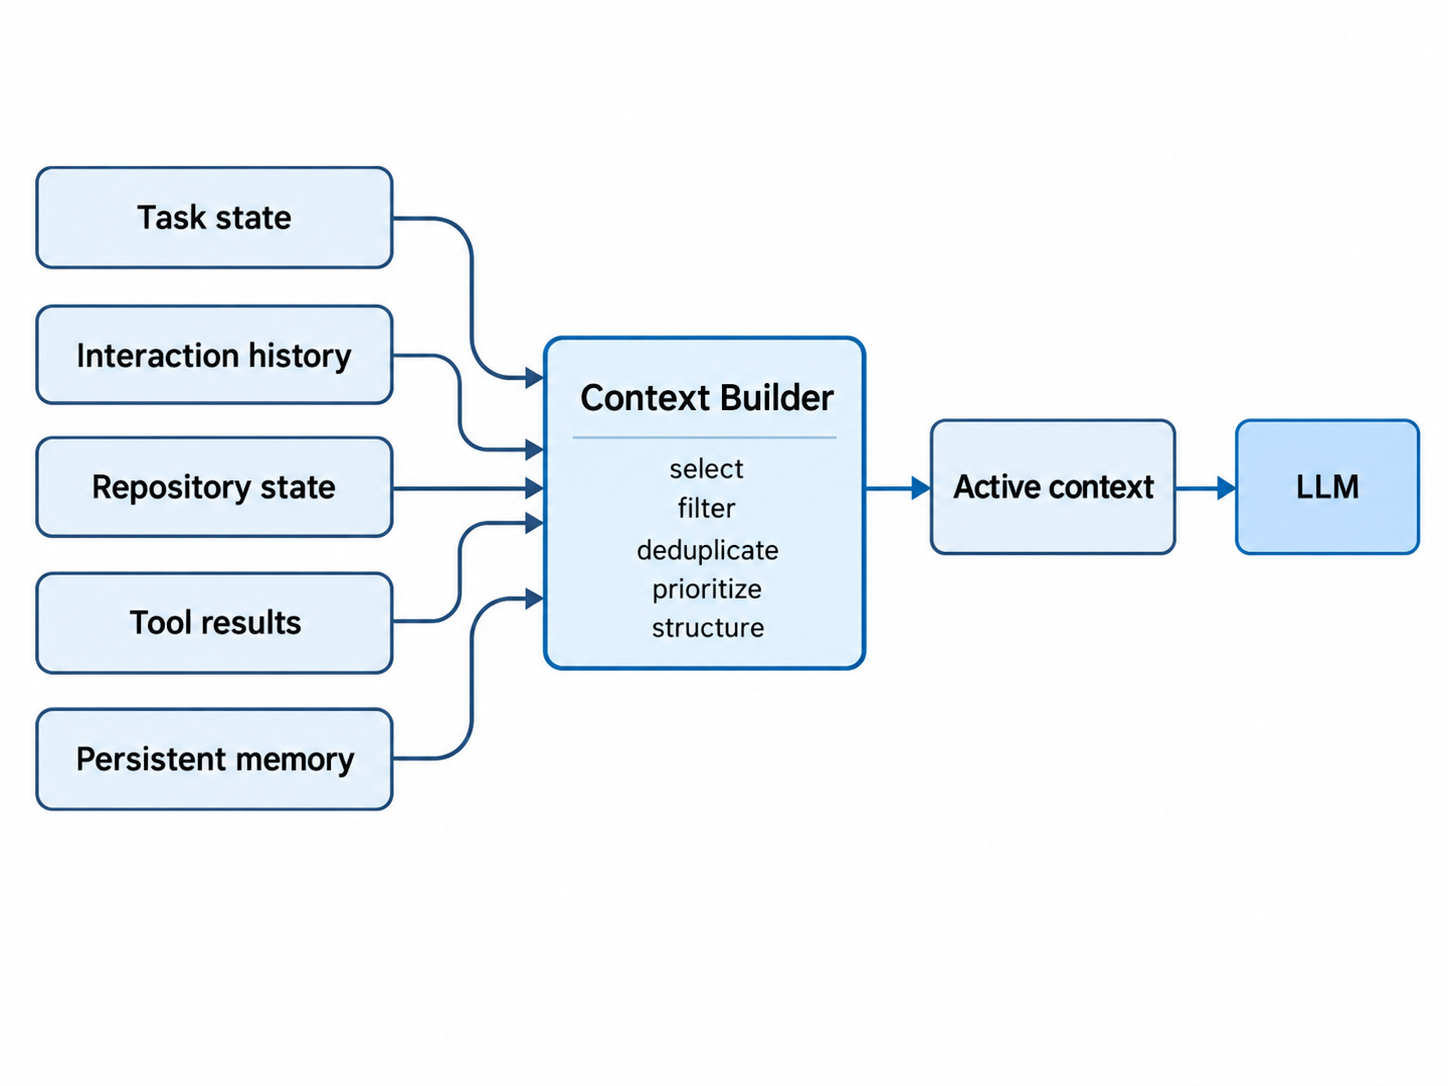
\includegraphics[width=\linewidth,trim=15bp 240bp 15bp 145bp,clip]{images/context-builder.png}
\captionsetup{hypcap=false}
\captionof{figure}{Construction of the active context from task state, interaction history, repository information, tool results and persistent memory.}
\label{fig:active-context-construction}
\end{minipage}

A context policy can distinguish information that should remain available throughout a task, such as the objective, explicit user constraints and relevant project rules, from information selected dynamically for the current step. Excluded detail should remain recoverable from its original source if it later becomes relevant.

Consider the recurring task \emph{Fix GitHub issue \#42 and verify the solution}. Initially, the active context may contain the issue description, project instructions and tools such as \texttt{search\_code}, \texttt{read\_file}, \texttt{apply\_patch} and \texttt{run\_tests}. If the issue concerns incorrect handling of an \texttt{Authorization} header, a code search may identify \texttt{src/auth.py} and related tests. After these files have been inspected, the complete search output may be replaced by the relevant source code, observed behaviour and current hypothesis. After a patch, the current diff and verification state become more important than earlier exploratory results.

Context construction is therefore iterative. Each tool interaction changes the available state and may change which information is useful for the next inference step. Tool interfaces should support this by filtering, paginating or limiting low-value output, while excessively broad or overlapping tool sets can also consume context and make tool selection more ambiguous \parencite{anthropic2025tools}.

A larger supported context window does not remove the need for selection. In the models and tasks evaluated by \textcite{liu2024lostmiddle}, the position of relevant information affected performance, with information in the middle of long contexts often being used less reliably. RULER likewise observed degradation with increasing sequence length and task complexity in the evaluated models \parencite{hsieh2024ruler}. Maximum context length should therefore be treated as a capacity limit rather than a target.

These choices also form part of the context policy introduced in Chapter~\ref{chap:benchmarks} and should remain controlled when candidate models are compared.

\section{History, task state and persistent memory}
\label{sec:history-memory}

Long-running tool interaction requires distinguishing different roles of retained information. Interaction history records what happened, task state represents information needed to continue the current task, and persistent memory refers here to selected information retained for reuse beyond the immediate task state. These are functional roles rather than mutually exclusive storage mechanisms; history and task state may themselves also be persisted.

The complete interaction history can contain messages, tool calls, raw search results and repeated test runs. It may remain available to the assistant runtime for audit, debugging or later retrieval without being included in every model request. Stored history and active context are therefore separate architectural concerns.

Task state should preserve the information required to continue coherently, such as the current goal, user constraints, inspected files, applied changes and verification status. Some of this state consists of operational facts that the runtime can record directly. Other information, such as an assumed root cause, is a model-derived hypothesis. Storing a hypothesis in a structured checkpoint does not make it an observed fact.

Structured checkpoints should therefore preserve the status of the information they contain. They can record, for example, that \texttt{src/auth.py} was modified and a test was executed while keeping the suspected relationship between the change and issue \#42 explicitly marked as a hypothesis until verified.

Verification state is also tied to the code state that was tested. If relevant code is modified afterwards, an earlier passing test remains a valid historical observation but no longer verifies the current version and may need to be repeated.

Persistent memory retains selected information useful for future work, such as repository conventions or recurring project-specific procedures. In a Java project, the command used to run tests may be reusable knowledge, while an intermediate test failure is usually temporary task state. MemGPT illustrates the broader principle of treating the model context as a limited working tier while moving information between it and larger external storage \parencite{packer2023memgpt}.

Persistent memory therefore requires policies for retention, retrieval, update and invalidation. Provenance is important: if stored memory states that a project uses Java 17 while the current \texttt{pom.xml} specifies Java 21, the current repository state is the more authoritative source.

Treating every stored observation as reusable memory would create an increasingly noisy retrieval source, even if the complete interaction history remains useful as an archive. Persistent memory should therefore favour information that is stable, reusable and worth retaining.

\section{Compaction and context efficiency}
\label{sec:compaction-efficiency}

Even with selective context construction, long tool interactions can produce more useful history than should remain verbatim in every request. Compaction addresses this by replacing part of the previous context with a smaller representation that preserves the information required to continue the task.

For a software-engineering assistant, compacted state should retain the goal, explicit user constraints, scope boundaries, acceptance criteria, important findings, relevant source references, architectural decisions, modified files, verification results and unresolved problems. It should also preserve distinctions between observed facts, hypotheses and unverified interpretations. Obsolete search results, duplicated source snippets, superseded hypotheses and large intermediate logs can often be removed.

Anthropic describes compaction as preserving important decisions and unresolved work while discarding redundant information, including old tool results \parencite{anthropic2025context}. OpenAI likewise provides compaction for long-running interactions to reduce context while carrying forward state required by later turns \parencite{openai-compaction}.

Compaction is inherently lossy. A smaller representation reduces token usage and irrelevant information, but may discard details that later become useful. Structured checkpoints can reduce this risk for explicitly recorded operational facts, while the original interaction history can remain stored outside the active context for later recovery.

\noindent\begin{minipage}{\linewidth}
\centering
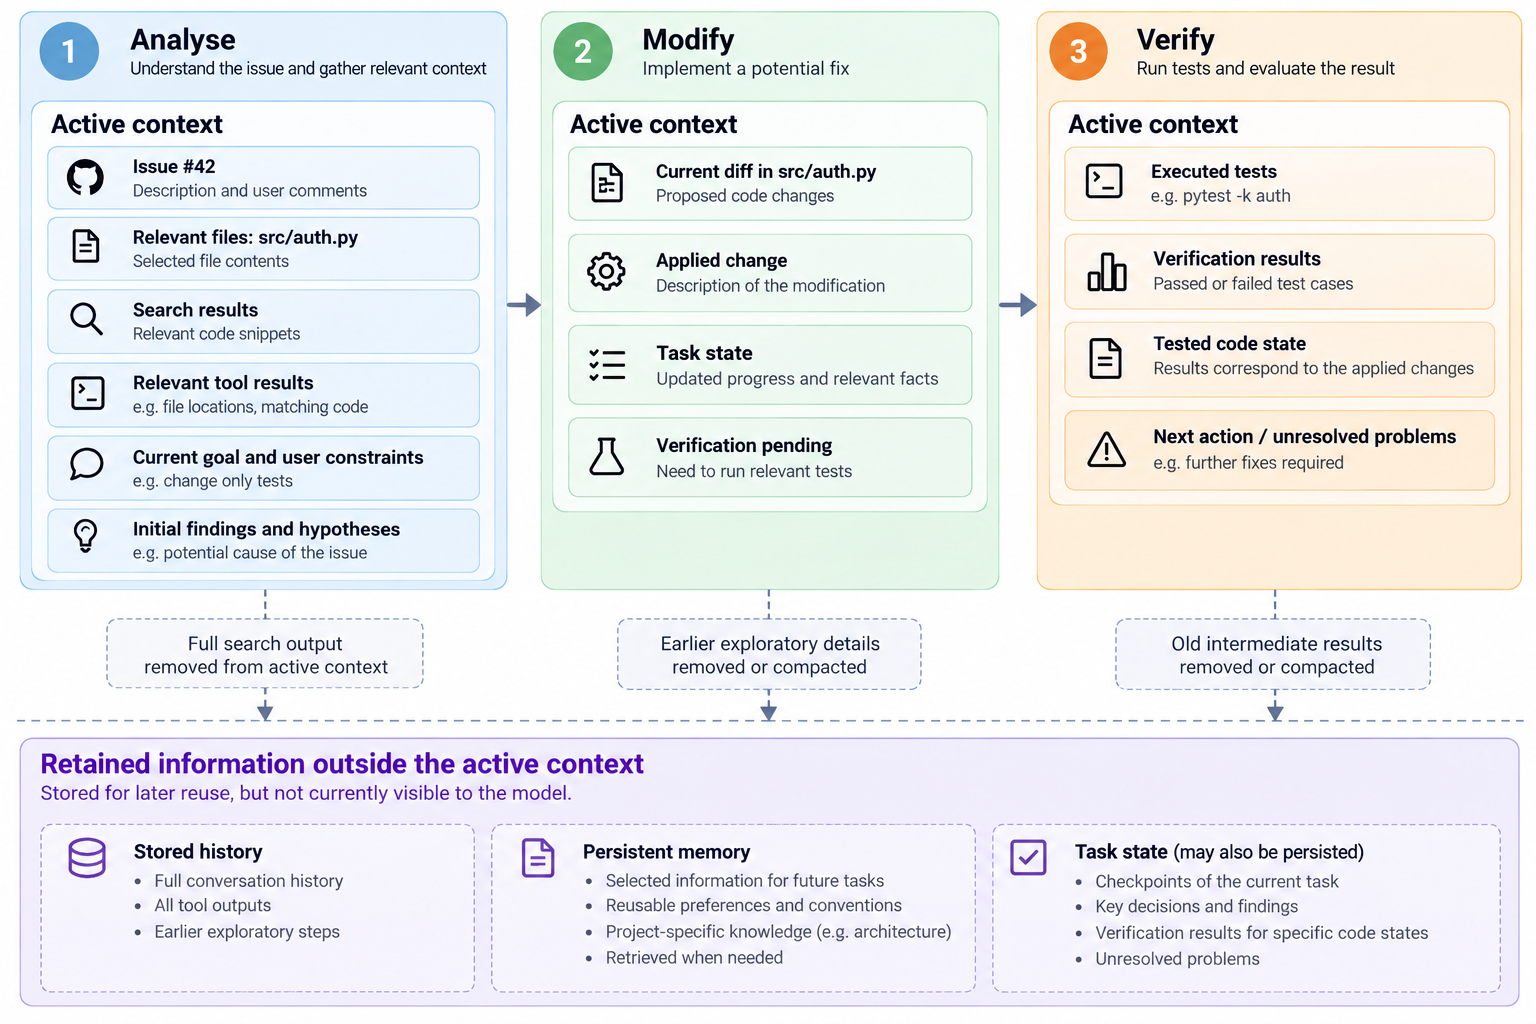
\includegraphics[width=\linewidth]{images/context-evolution.png}
\captionsetup{hypcap=false}
\captionof{figure}{Evolution of the active context while analysing, modifying and verifying GitHub issue \#42.}
\label{fig:active-context-evolution}
\end{minipage}

Prompt caching addresses a separate efficiency problem. The KV cache introduced in Chapter~\ref{chap:local-llms} stores attention key-value states during inference. Prompt caching can reuse previously computed states across model requests that share a cacheable prefix, although the exact mechanism depends on the runtime or API provider. Stable information such as system instructions, project rules and tool definitions can therefore benefit from repeated prefix reuse \parencite{openai-prompt-caching}.

Prompt caching does not increase context capacity. Cached input still occupies the model's context window; caching reduces repeated computation rather than the amount of information presented to the model. Persistent memory, compaction and prompt caching therefore solve different problems.

These mechanisms can also interact. Compaction may reduce input tokens but alter part of the previously reusable prefix, while an unchanged earlier prefix may remain cacheable. Context management is therefore an optimisation across model quality, context usage, latency and computational reuse rather than a simple attempt to minimise token count.

These considerations suggest an architecture in which the AI Software Engineering Assistant should maintain explicit task state, select information relevant to the current step, retrieve reusable persistent information when required and compact interaction history as a task grows. The remaining question is how the assistant can efficiently locate external information not already present in its active context. This leads to retrieval-augmented generation and agentic retrieval, examined in the following chapter.

% !TeX root = ../Tempel-Daniel.tex
\chapter{RAG and Agentic Retrieval}
\label{chap:retrieval}

The previous chapter established that the active context of the AI Software Engineering Assistant should contain information relevant to the model’s current decision rather than all information available to the runtime. A software repository creates the corresponding retrieval problem: a task may depend on only a few methods, tests or configuration files, while the complete repository may contain thousands of files. The challenge is therefore not simply to provide the LLM with more context, but to locate the external evidence relevant to the current task.

\textcite{lewis2020rag} introduced Retrieval-Augmented Generation (RAG) by combining parametric model knowledge with information retrieved from an external non-parametric source. The original work used a neural retriever and dense index. This chapter uses RAG in the broader architectural sense common in current LLM systems: generation is augmented with externally retrieved information at inference time. For a software-engineering assistant, such sources can include repository files, documentation and project knowledge that change independently from model parameters.

\section{Repository-aware retrieval}
\label{sec:repository-retrieval}

Retrieval does not necessarily require a separately constructed vector index. Direct text or symbol search can operate on current repository files, while indexed systems prepare searchable representations in advance. The appropriate approach depends on repository size, task requirements and measured retrieval quality.

Indexed retrieval typically divides source material into searchable units and associates them with metadata such as file path, module, class or symbol. Source code makes this more difficult than prose because useful information follows program structure rather than arbitrary token boundaries. Structure-aware chunking can preserve boundaries such as functions or methods, but retrieval units must remain small enough to search efficiently while retaining enough surrounding information to be interpretable.

Repository search can use several relevance signals. Lexical retrieval is effective for exact identifiers, exception names, configuration keys or error messages. BM25 is a widely used lexical ranking method and remains a strong baseline across heterogeneous retrieval tasks \parencite{thakur2021beir}.

Lexical overlap becomes less reliable when the task and implementation use different terminology. A user may describe authentication behaviour while the repository represents it through identifiers such as \texttt{validateBearerToken} or \texttt{securityContext}. Dense retrieval addresses this mismatch by representing queries and searchable units as embeddings. CodeSearchNet illustrates this problem directly: semantic code search must connect natural-language descriptions with the technical vocabulary used in source code \parencite{husain2019codesearchnet}.

Repository structure can provide another useful signal. Source files are connected through calls, imports, symbol references, inheritance and test–implementation relationships. If retrieval identifies a function in \texttt{src/auth.py}, its callers, validation helpers or related tests may be more useful than unrelated code with similar wording. RepoGraph explores this principle by representing repository-level relationships as a graph for AI software-engineering tasks \parencite{ouyang2025repograph}. Such structural information requires additional analysis and may be incomplete.

Lexical, dense and structural retrieval should therefore be treated as complementary options rather than mandatory stages. A retrieval subsystem can select or combine them according to the repository, task and evaluation results. An indexed system may also retrieve a broad candidate set and then apply a reranker to a smaller subset. A reranker may improve ranking quality at additional computational cost \parencite{thakur2021beir}.

Figure~\ref{fig:rag-agentic-retrieval} shows direct and indexed routes to repository evidence; the feedback path allows further retrieval when the current evidence is insufficient.

\begin{figure}[!htbp]
\centering
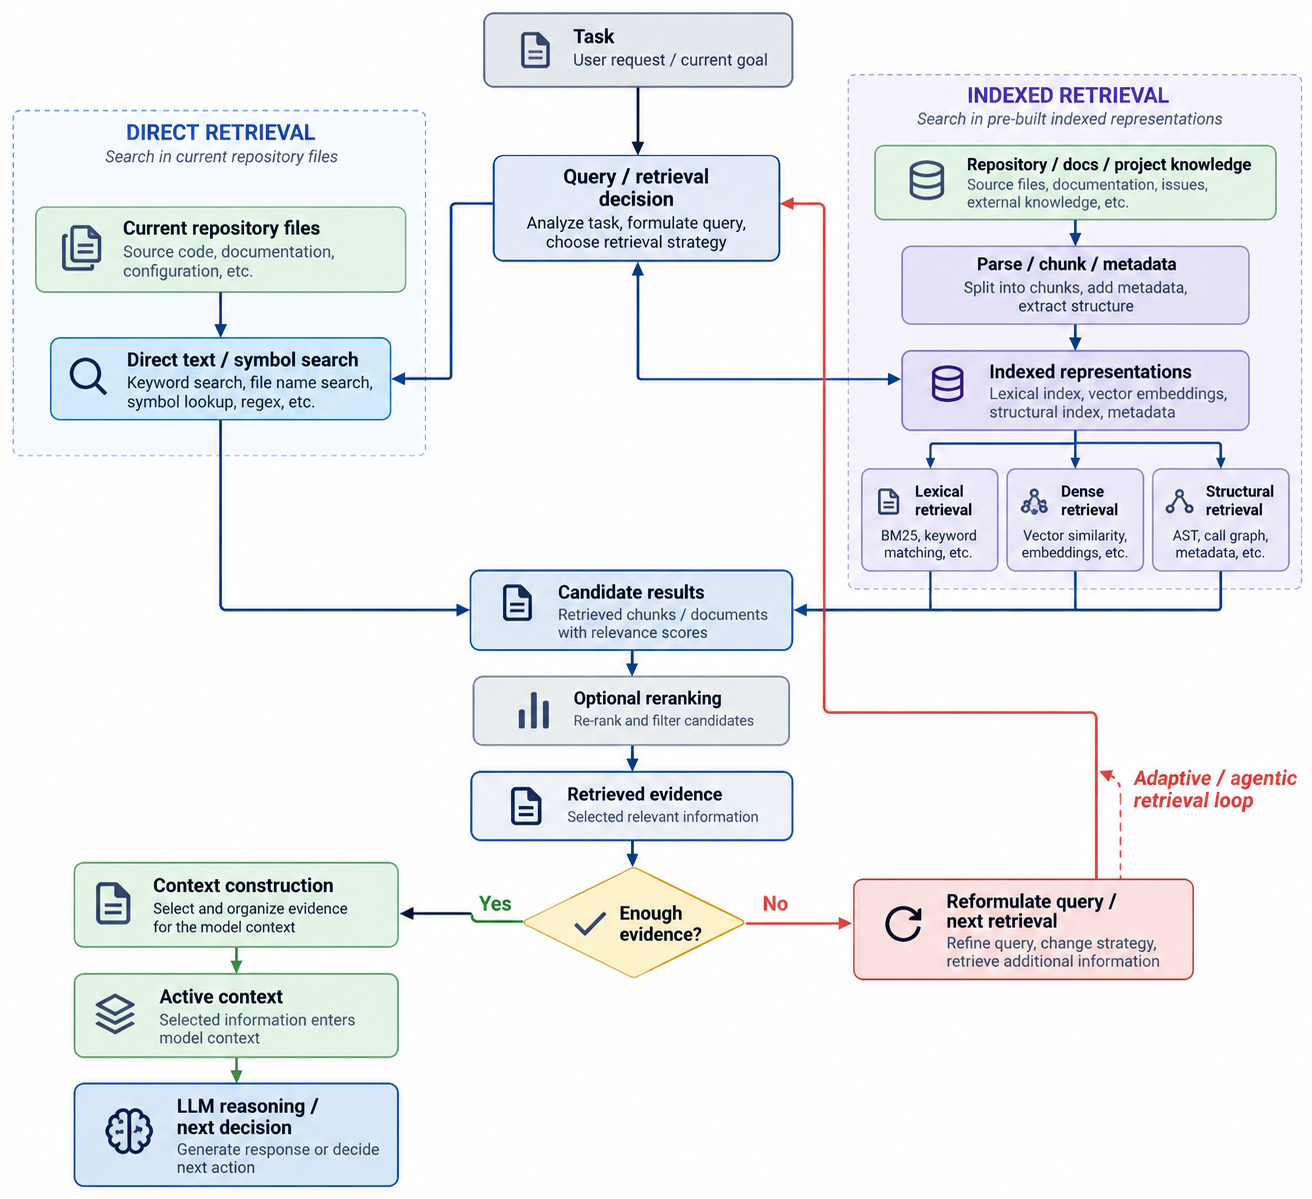
\includegraphics[width=\linewidth]{images/rag-agentic-retrieval.png}
\caption{Direct and indexed repository retrieval for the AI Software Engineering Assistant, including optional lexical, dense and structural search, reranking and adaptive additional retrieval.}
\label{fig:rag-agentic-retrieval}
\end{figure}

\noindent\begin{minipage}{\linewidth}
Table~\ref{tab:retrieval-signals} summarises the uses and limitations of these complementary retrieval signals.\par\vspace{5pt}
\captionsetup{hypcap=false}
\captionof{table}{Retrieval signals for repository tasks and their typical limitations.}
\label{tab:retrieval-signals}
\small\singlespacing
\renewcommand{\arraystretch}{1.15}
\begin{tabular}{@{}p{2.7cm}p{6.0cm}p{6.8cm}@{}}
\toprule
{\raggedright\textbf{Retrieval signal}\par} & {\raggedright\textbf{Useful for repository tasks}\par} & {\raggedright\textbf{Typical limitation}\par} \\
\midrule
{\raggedright Lexical retrieval\par} & {\raggedright Exact symbols, identifiers and error messages\par} & {\raggedright Limited when query and implementation use different terminology\par} \\
{\raggedright Dense retrieval\par} & {\raggedright Semantic similarity between natural language and source code\par} & {\raggedright May rank semantically related but incorrect identifiers highly\par} \\
{\raggedright Structural retrieval\par} & {\raggedright Calls, imports, references and test–implementation relationships\par} & {\raggedright Requires additional analysis and may be incomplete\par} \\
\bottomrule
\end{tabular}
\end{minipage}

Retrieved results should be treated as external evidence rather than as the complete model context. For the recurring task \emph{Fix GitHub issue \#42 and verify the solution}, an initial search for \texttt{Authorization} may locate \texttt{src/auth.py} and related tests. These results can then be passed to the context-building stage described in Chapter~\ref{chap:context-memory} together with the issue description and current task state.

\section{From iterative retrieval to agentic retrieval}
\label{sec:agentic-retrieval}

{\setlength{\emergencystretch}{2em}
A single retrieval operation is sufficient when the information need is already clear. Repository-level tasks are often less direct because an issue describes observed behaviour while relevant implementation details become visible only after part of the repository has been inspected.\par}

Suppose issue \#42 reports that an \texttt{Authorization} header is handled incorrectly. The assistant may first search for \texttt{Authorization} and inspect \texttt{src/auth.py}. That file may reveal a separate token-validation function, whose implementation and references lead to middleware configuration or tests defining the expected behaviour. The useful search sequence therefore cannot always be formulated completely from the original issue description.

This creates an iterative process:

\begin{center}
\small\singlespacing
search \(\rightarrow\) inspect evidence \(\rightarrow\) identify missing information
\\ \(\rightarrow\) reformulate the search \(\rightarrow\) retrieve again.
\end{center}

RepoCoder applies a related principle to repository-level code completion by alternating retrieval and generation. Its experiments showed improvements over the vanilla retrieval-augmented baseline evaluated in that work \parencite{zhang2023repocoder}. This supports iterative use of newly discovered information, but does not by itself demonstrate the benefit of autonomous retrieval decisions for issue-resolution tasks.

Iteration alone does not make retrieval agentic. A fixed pipeline could always perform several searches without making adaptive decisions. Here, \textbf{agentic retrieval} refers to retrieval in which subsequent search decisions depend on intermediate evidence. The model or surrounding runtime can decide whether another search is required, what information is missing, which retrieval mechanism to use and when sufficient evidence has been collected.

Recent work on Agentic RAG describes a broader transition from fixed pipelines toward systems that adapt retrieval strategies and refine queries across multiple evidence-gathering steps \parencite{singh2025agenticrag}. Agentic retrieval refers here to the retrieval component of this behaviour, while Agentic RAG describes the wider interaction between adaptive retrieval, generation and reasoning.

Adaptive steps may combine direct text or symbol search with indexed lexical, dense or structural retrieval. Editing, testing and task completion belong to the broader agent loop described in Chapter~\ref{chap:agents}.

Adaptive retrieval adds cost and failure modes. Query reformulation can drift away from the original task, repeated searches can return the same evidence and unnecessary retrieval rounds increase latency and model usage. A failed search also does not establish that no relevant implementation exists; another query or retrieval method may still locate it. Retrieval budgets and tracking of previously inspected results can therefore limit unnecessary search.

\section{Retrieval reliability}
\label{sec:retrieval-reliability}

Retrieval quality depends not only on relevance but also on whether the retrieved information corresponds to the repository state on which the assistant operates. An index is a derived representation of repository content and can become stale when files change.

Repository, branch and commit metadata can identify the source snapshot from which indexed information was produced. A commit, however, does not represent uncommitted working-tree changes. Because operations such as \texttt{apply\_patch} modify files before a new commit necessarily exists, relevant indexed results should be checked against the current working-tree files before they are used to justify an edit.

Incremental indexing can update affected entries and relationships after files are added, modified or deleted rather than rebuilding the complete index after every change. Structural indexes require particular care because a change in one file can alter relationships to symbols elsewhere.

Not every form of current state belongs in a retrieval index. Frequently changing operational information such as Git status, test output or CI results can be obtained directly through tools. Retrieval is more appropriate for searching larger collections of source code, documentation and project knowledge.

Retrieval should also be evaluated separately from the LLM that consumes its results. A failure caused by missing evidence differs from one in which correct evidence was retrieved but interpreted incorrectly. Retrieval can also succeed while the context-building stage excludes the relevant result. Component-level evaluation therefore helps distinguish these failure sources by recording both retrieved evidence and the information actually included in the active context.

For a single ranked retrieval operation, Recall@k measures the proportion of annotated relevant retrieval units found among the top-k results. The retrieval unit may be a file, method or chunk and must be defined together with the relevance labels used by the evaluation set. A ranking metric such as nDCG@k can additionally account for graded relevance and result position.

An agentic retrieval strategy may execute several queries and combine evidence across multiple steps. It should therefore also be evaluated at task level under a defined retrieval or tool budget. Relevant measures include whether the required evidence was eventually acquired, retrieval latency, the number of retrieval rounds and, ultimately, whether the complete assistant succeeds on realistic software-engineering tasks.

Repository characteristics and evaluation results should determine which retrieval mechanisms and degree of adaptation are useful. The following chapter examines the Model Context Protocol as a standardised interface for exposing repository resources and retrieval tools to the assistant runtime.

% !TeX root = ../Tempel-Daniel.tex
\chapter{Model Context Protocol}
\label{chap:mcp}

The previous chapters established that the AI Software Engineering Assistant may need to retrieve repository information and invoke operations such as reading source files, running tests and interacting with GitHub. Each external system still requires backend-specific integration code, and equivalent integrations may otherwise need to be implemented separately for different AI applications.

The Model Context Protocol (MCP) addresses this problem by defining a shared protocol through which compatible applications can access externally provided data and operations. MCP does not eliminate backend-specific integration code; it places that code behind a reusable protocol boundary. This responds to the original MCP motivation of reducing fragmented integrations between AI applications and external data sources and tools \parencite{anthropic2024mcp}.

\section{Standardising external capabilities}
\label{sec:mcp-capabilities}

In MCP terminology, the AI Software Engineering Assistant acts as the \textbf{Host}. The Host manages MCP clients that communicate with MCP servers, while each server exposes capabilities backed by an underlying system such as GitHub, a repository, a database or another service \parencite{mcp2026architecture}.

Figure~\ref{fig:mcp-architecture} shows how the Host\textquotesingle s MCP clients connect the assistant to external systems through servers responsible for their backend integrations.

\begin{figure}[!htbp]
\centering
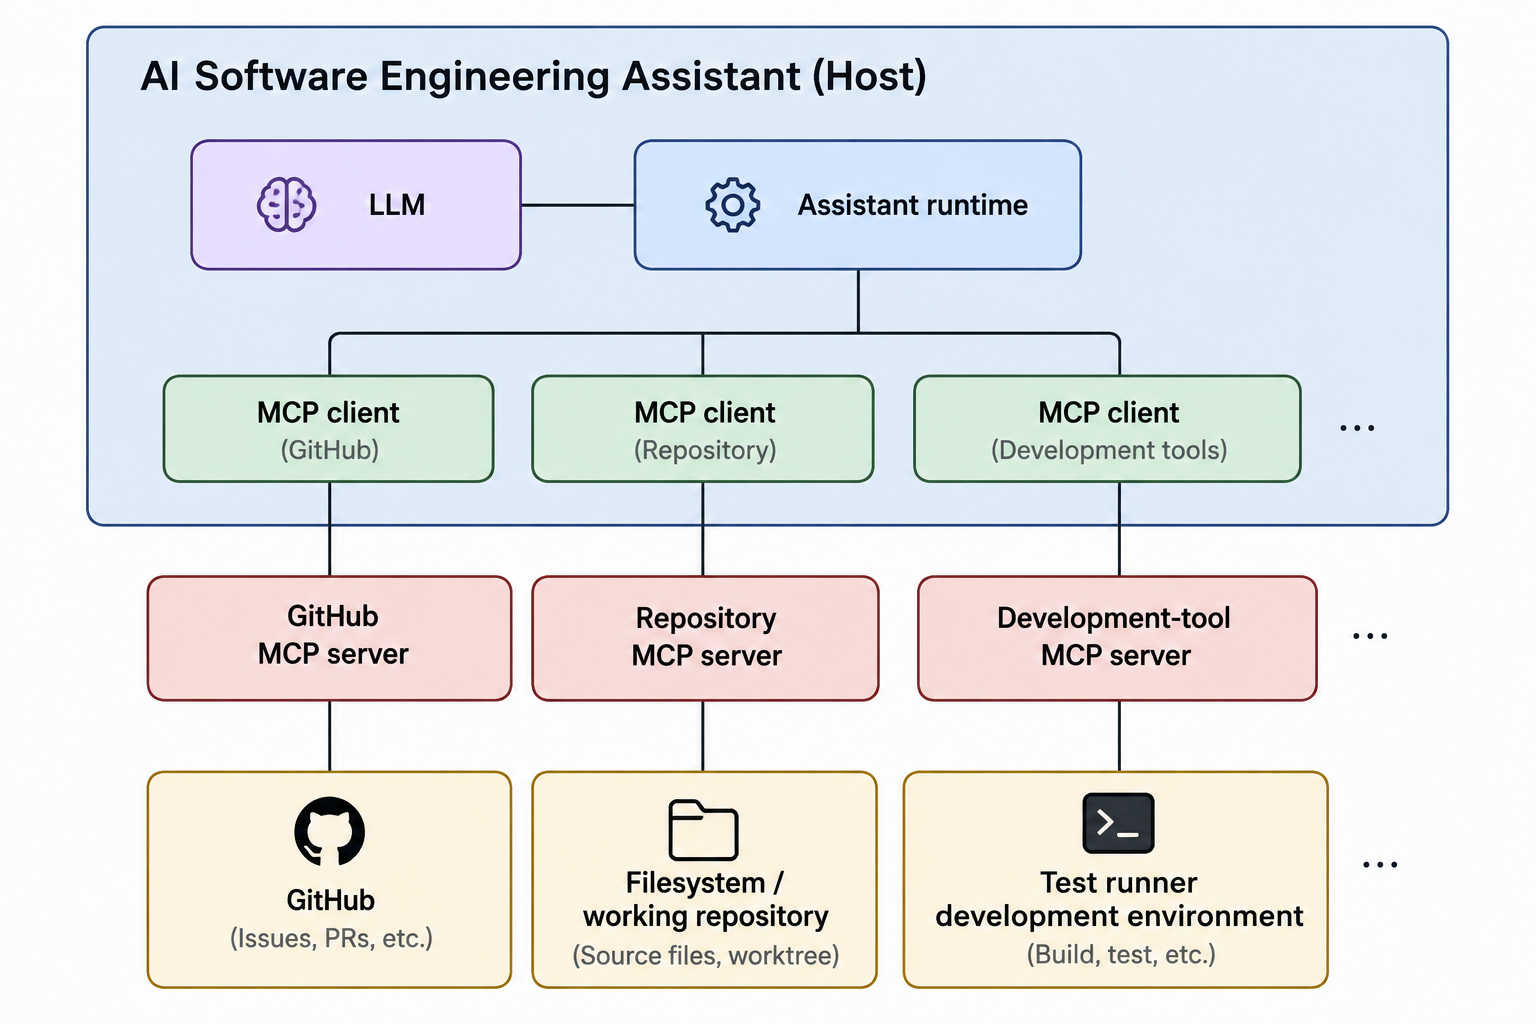
\includegraphics[width=\linewidth]{images/mcp-host-client-server.png}
\caption{Placement of MCP clients and servers between the AI Software Engineering Assistant and external systems.}
\label{fig:mcp-architecture}
\end{figure}

These server connections expose capabilities as \textbf{tools}, \textbf{resources} and \textbf{prompts}. Tools represent invocable operations, resources provide addressable data, and prompts provide reusable message templates. For the software-engineering workload considered here, tools and resources are most relevant because they provide access to executable operations and repository-related information.

MCP tool discovery should be distinguished from the tool-calling interface of the LLM. A server can describe a tool through its name, description and schema, but the model does not communicate with the MCP server directly. The Host selects which discovered tools are made available to the model and maps their definitions to the tool-calling interface of the selected inference runtime or model API. If the LLM generates a structured call such as \texttt{search\_code("Authorization")}, the assistant runtime maps it back to the corresponding MCP server. MCP therefore complements the function calling described in Chapter~\ref{chap:tool-use} rather than replacing it.

Figure~\ref{fig:mcp-tool-flow} follows a model-generated request through Host validation and MCP routing to backend execution, then returns the result for a subsequent model request.

\begin{figure}[!htbp]
\centering
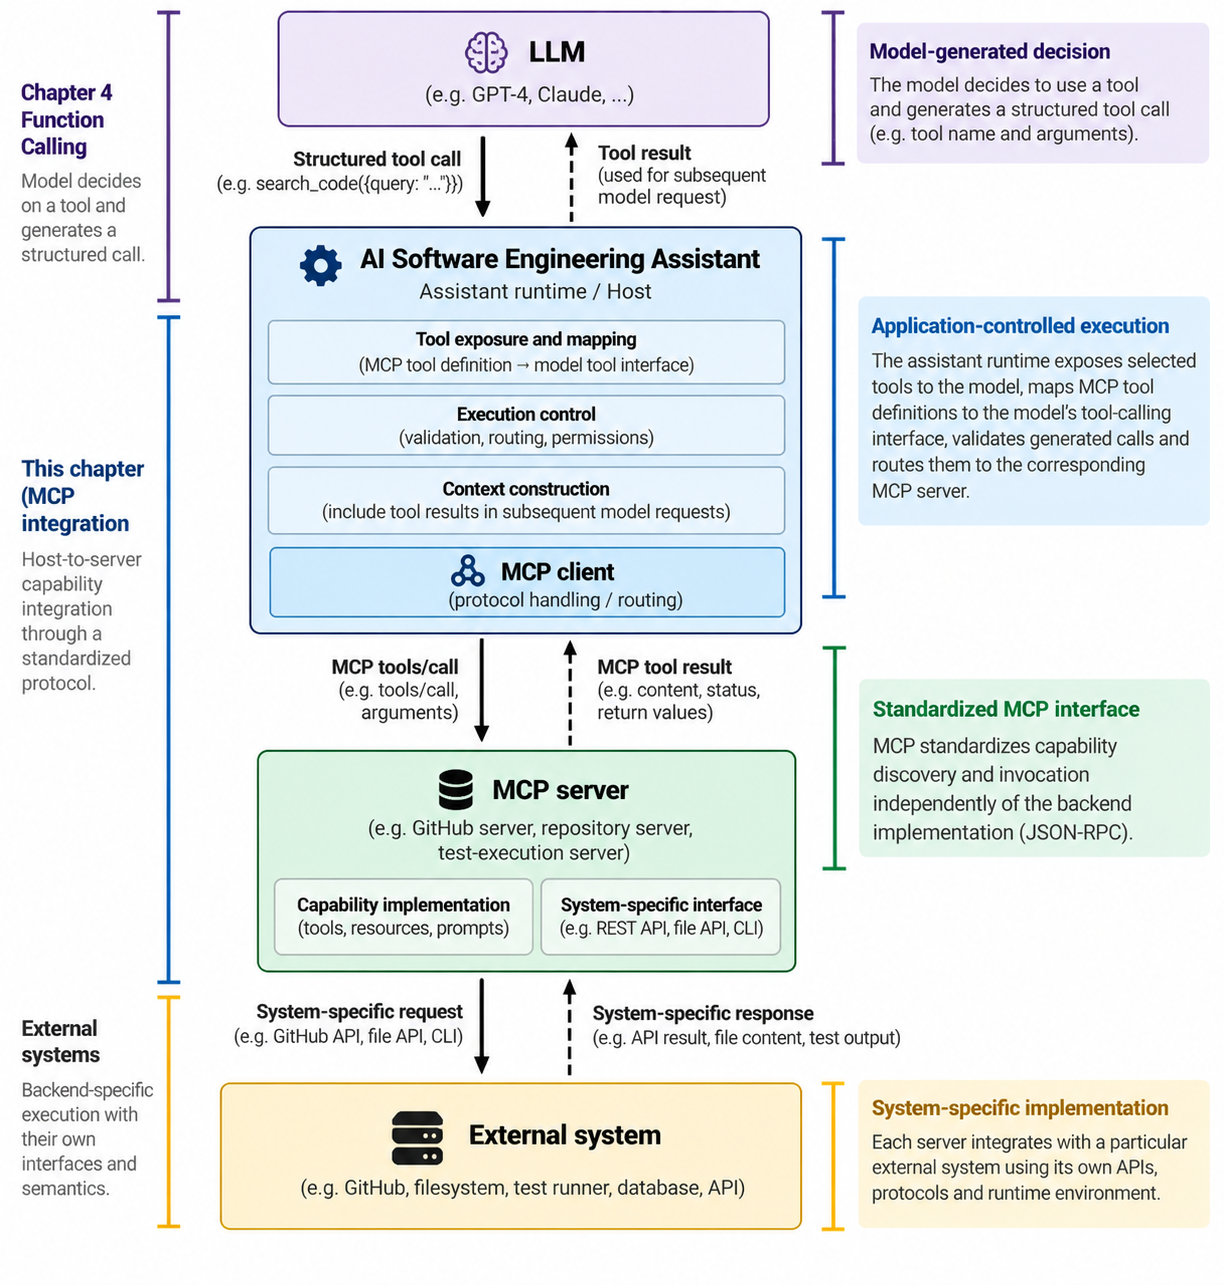
\includegraphics[width=\linewidth]{images/mcp-tool-execution-flow.png}
\caption{Flow from MCP tool discovery through model-visible tool selection to external tool execution and returned results.}
\label{fig:mcp-tool-flow}
\end{figure}

The set of capabilities exposed by a server, the subset selected by the Host and the tools actually included in a model request are separate concerns. When tool definitions are included in model requests, selecting a smaller task-relevant subset can reduce active-context usage and tool-selection ambiguity.

MCP uses JSON-RPC and supports both local and remote servers. This chapter refers to protocol revision \texttt{2026-07-28}, whose core uses self-contained requests rather than the protocol-level session lifecycle of earlier revisions \parencite{mcp2026architecture}. A stateless protocol core does not require the server or its operations to be stateless.

\section{MCP in the software engineering assistant}
\label{sec:mcp-assistant}

Consider again the task \emph{Fix GitHub issue \#42 and verify the solution}. The assistant needs the issue description, relevant repository information, the ability to modify the implementation and a way to verify the resulting code state. These capabilities may originate from independent systems while still being exposed through MCP.

A GitHub MCP server could provide operations for reading issue \#42 and creating a pull request. A repository or filesystem server could expose \texttt{read\_file}, \texttt{search\_code} and \texttt{apply\_patch}, while a test-execution MCP server could expose \texttt{run\_tests}. This allows heterogeneous backends to participate in one workflow without requiring the assistant runtime to implement each backend protocol directly.

A shared protocol does not create a shared workspace automatically. If repository inspection, modification and testing are handled by different servers, the Host must ensure that they refer to the intended repository, branch or working copy and to a consistent code state. A successful test result is relevant only if it verifies the version containing the changes being evaluated.

GitHub's official MCP server illustrates this approach by exposing GitHub functionality through configurable toolsets and individual tools. It can also operate in read-only mode, removing write operations exposed through that server \parencite{github-mcp-configuration}. Such configuration limits the GitHub integration but does not restrict capabilities provided by other independently configured servers.

MCP access should also be distinguished from retrieval and context construction. A server may expose a \texttt{search\_code} tool, but MCP does not define whether the underlying retrieval uses lexical search, embeddings or another strategy. Similarly, information returned through MCP does not automatically enter the LLM's active context. The assistant's context policy still determines which results are included, summarised or retained. MCP therefore standardises access, while retrieval determines what is found and context engineering determines what the model receives.

The same distinction applies to backend semantics. A GitHub MCP server may translate a tool call into GitHub API operations, while a filesystem server uses file APIs and a test-execution server starts a build or test process. MCP standardises capability exposure and invocation, not the behaviour of the underlying systems.

\section{Benefits, boundaries and production trade-offs}
\label{sec:mcp-tradeoffs}

The main architectural benefit of MCP is \textbf{reuse through a common integration boundary}. Backend-specific adapters still have to be implemented, but an MCP server can expose them to multiple compatible Hosts. Machine-readable discovery also allows a Host to obtain capability definitions without hard-coding every externally provided operation.

Protocol compatibility does not imply semantic uniformity. Two MCP servers may provide repository-search tools with different names, schemas, result structures or behaviour. Clear tool descriptions, bounded responsibilities and predictable results therefore remain important; MCP standardises the interaction mechanism but does not guarantee the quality of the interface.

The additional protocol boundary also introduces costs. Remote servers can add network latency, while separately deployed components introduce additional failure, versioning and observability concerns. These costs are useful when reuse or independent deployment matters, but a small system with a few fixed local operations may remain simpler with direct function integration.

MCP compatibility alone also does not establish a security boundary or make a connected server trustworthy. Isolation, authorisation and input validation must be enforced by the Host, server and deployment environment. Local servers are not automatically sandboxed, capabilities should follow least-privilege principles, and sensitive operations may require Host-controlled user approval \parencite{mcp2026security}.

MCP provides a reusable integration boundary through which heterogeneous external capabilities become available to the assistant. Coordinating those capabilities toward a task objective is the responsibility of the agents and agent harnesses examined in the following chapter.

% !TeX root = ../Tempel-Daniel.tex
\chapter{AI Agents and Agent Harnesses}
\label{chap:agents}

The previous chapters established the components required for the AI Software Engineering Assistant to construct context, retrieve repository information and request external operations through structured tool calls, which the runtime may route through MCP. These capabilities do not by themselves coordinate multiple actions toward a task objective.

A request such as \emph{Fix GitHub issue \#42 and verify the solution} may require inspection, modification, testing and further investigation based on intermediate results. In this report, an \textbf{agent} is a system in which an LLM selects actions toward a task objective, while an \textbf{agent harness} executes and constrains those actions, maintains operational state and returns observations for subsequent decisions.

\section{From tool calls to an agent loop}
\label{sec:agent-loop}

An \textbf{agent loop} extends the tool interaction described in Chapter~\ref{chap:tool-use} across a task. Figure~\ref{fig:agent-loop} shows how the harness constructs context, invokes the model, dispatches accepted actions and updates task state before deciding whether another iteration is permitted.

\begin{center}
\begin{minipage}{\linewidth}
\centering
\captionsetup{hypcap=false}
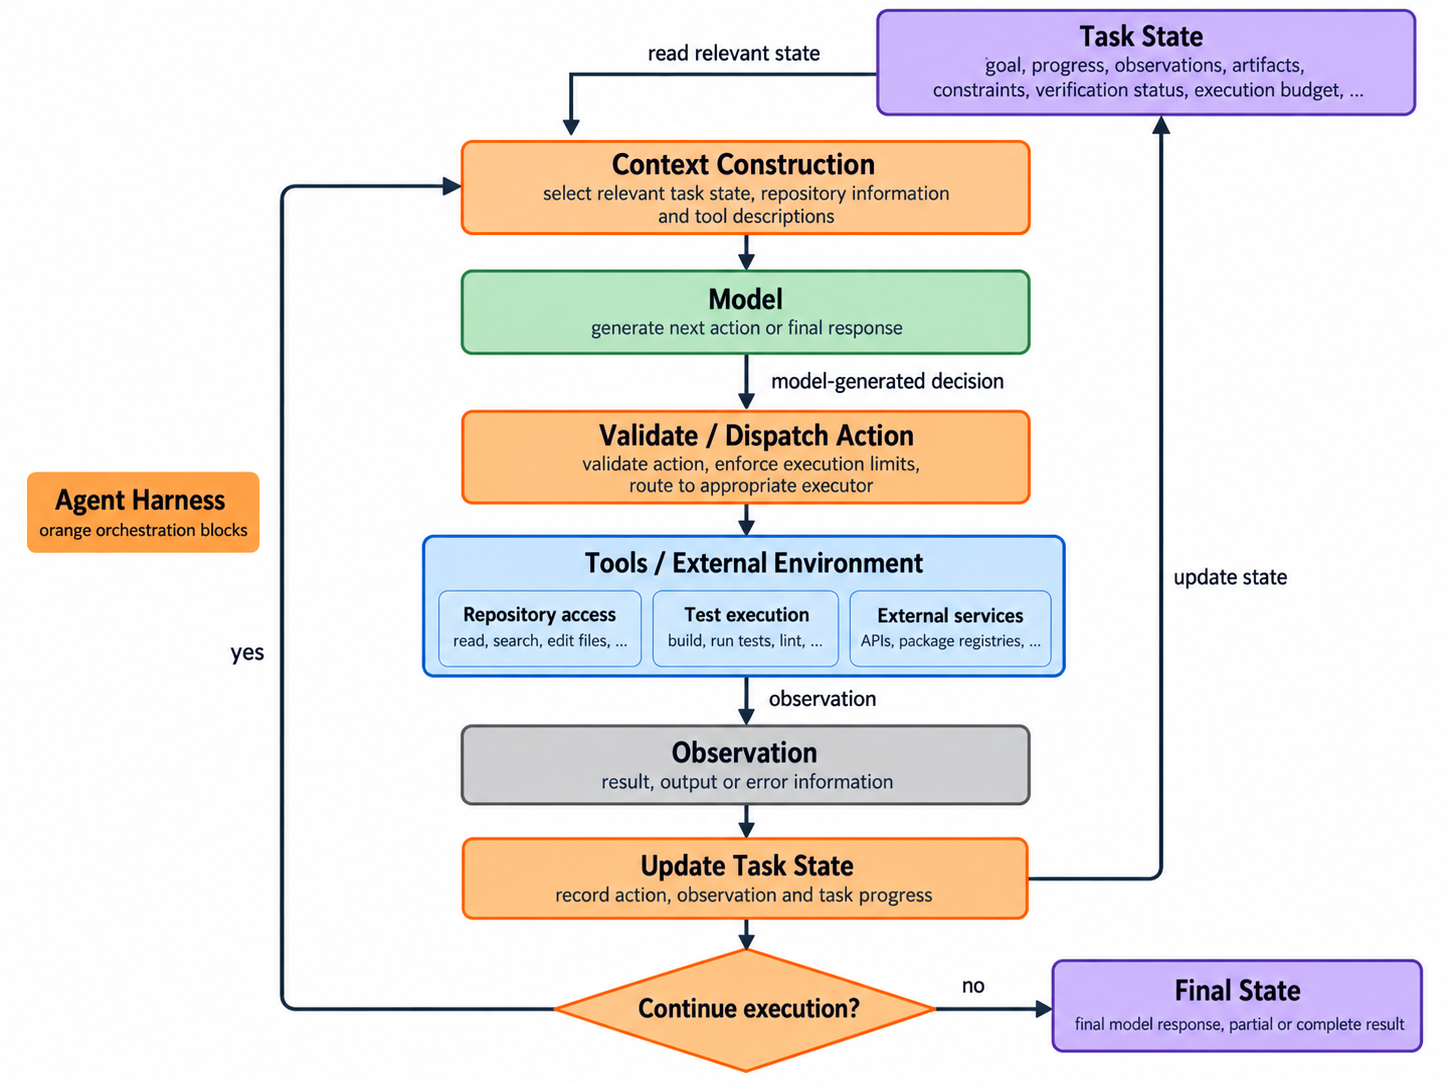
\includegraphics[width=\linewidth]{images/agent-loop-harness.png}
\captionof{figure}{Agent loop in which the model selects subsequent actions while the agent harness constructs context, dispatches actions, updates task state and controls continuation. Termination of the loop does not by itself establish successful task completion.}
\label{fig:agent-loop}
\end{minipage}
\end{center}

The return path supplies updated observations for the next model decision; leaving the loop does not itself establish task success. If \texttt{run\_tests} executes correctly but reports failing assertions, the result is a useful observation that may lead to further inspection or another modification. Failure to start the test process or a timeout instead represents an execution problem and may require runtime-level recovery.

A workflow may also branch according to intermediate results while following predefined orchestration rules. In the agent loop considered here, the model has greater freedom to select and sequence subsequent actions within limits enforced by the harness. Real systems can combine both approaches. Anthropic similarly distinguishes predefined workflows from agents that dynamically direct their own tool usage \parencite{schluntz2024agents}.

This interaction is related to the action–observation structure of ReAct, where external actions provide evidence for subsequent model decisions \parencite{yao2023react}. Interface design also matters. SWE-agent demonstrates through its \textbf{Agent-Computer Interface (ACI)} that the behaviour and feedback of repository navigation, editing and execution tools can materially affect agent performance \parencite{yang2024sweagent}.

\section{Task state, recovery and completion}
\label{sec:agent-task-state}

Multi-step execution requires a coherent \textbf{task state} independent of the active model context. Relevant state can include the task objective, progress, modified artefacts, observations, verification status and execution budget. Only the subset needed for the next decision has to enter the active context.

State should reflect its source. Execution and verification status should be updated from runtime-observed results: requesting \texttt{apply\_patch} does not mean that a file was modified, and a model statement that tests passed is not a verification result. Model-generated plans and root-cause hypotheses remain inferred information until supported by observations.

Failure handling occurs at different levels. A transient infrastructure problem may justify a bounded \textbf{runtime retry} of the same operation. A compiler error or failing assertion produced by a successfully executed tool instead becomes an observation for \textbf{model-driven recovery}, in which the model changes its strategy or gathers additional evidence.

Side-effecting operations require additional care. If \texttt{create\_pull\_request} succeeds but its response is lost, blindly repeating the request may create a duplicate. The runtime should determine the previous outcome when possible. If this cannot be established, task state should preserve the uncertainty and automatic repetition may need to stop.

The harness also enforces execution budgets and stopping policies. When the model signals completion, the harness records whether available evidence satisfies the defined acceptance criteria. Missing or failed verification must remain distinguishable from verified completion. Longer tasks may additionally use checkpoints so that execution can resume after interruption; production persistence is addressed in the following chapter.

\section{Delegation and subagents}
\label{sec:agent-delegation}

A \textbf{subagent} is an additional agent assigned a bounded delegated task and a selected context. For issue \#42, Figure~\ref{fig:agent-delegation} shows parallel investigation of tests, code and recent changes, followed by integration, modification and verification by the main agent.

\begin{center}
\begin{minipage}{\linewidth}
\centering
\captionsetup{hypcap=false}
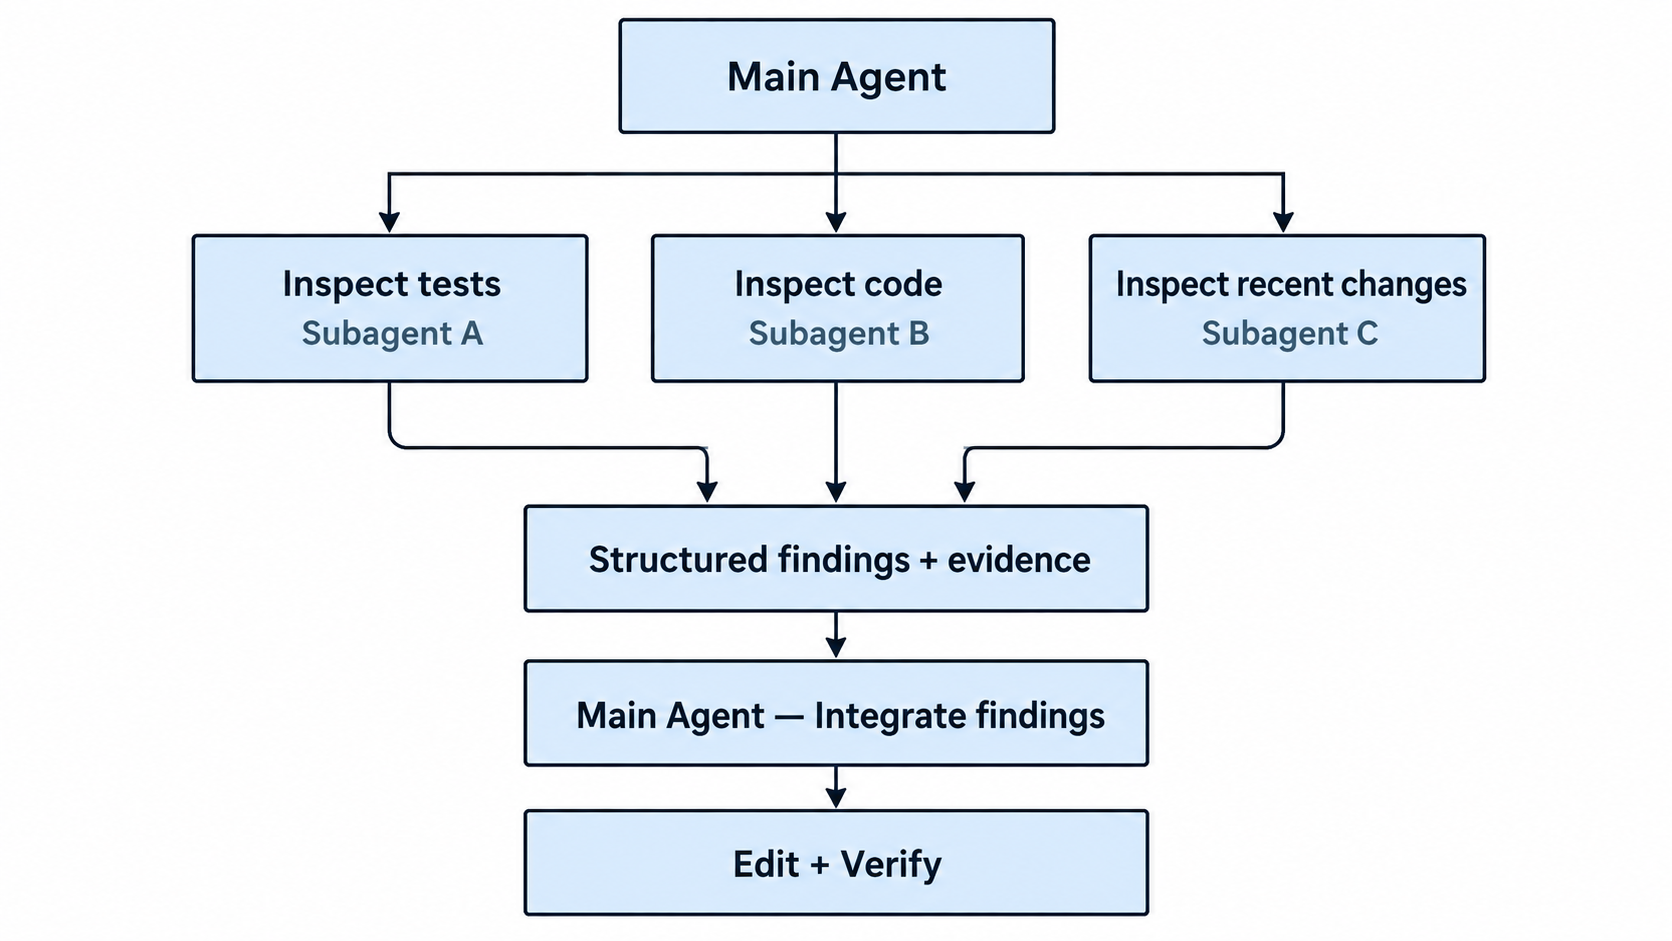
\includegraphics[width=0.88\linewidth]{images/agent-subagent-delegation.png}
\captionof{figure}{Delegation of independent investigation tasks to subagents, followed by centralised integration and verification by the main agent.}
\label{fig:agent-delegation}
\end{minipage}
\end{center}

Subagents can reduce context interference because each receives only information relevant to its task, and logically independent investigations may execute concurrently. Anthropic applies a related pattern in its multi-agent research system, where a lead agent delegates independent research directions and later combines their results \parencite{hadfield2025multiagent}.

Logical independence does not guarantee lower latency. Several subagents sharing a constrained local inference backend may compete for the same compute resources. Delegated findings should therefore be useful even without parallel speedup and retain enough provenance to identify the inspected code state and supporting observations.

Parallel modification of shared repository state creates additional coordination problems because agents may operate on outdated assumptions or produce conflicting edits. For the assistant considered here, a conservative pattern is to use subagents primarily for independent investigation while the main agent performs integration, code modification and final verification.

The harness tracks delegated work and enforces predefined failure and budget policies, while the main agent evaluates conflicting findings and decides whether further investigation is required.

Agent harnesses therefore connect model decisions, context, tools and task state into adaptive multi-step execution, while subagents add bounded delegation where useful. Deploying this execution model reliably introduces separate concerns such as model routing, long-running task persistence, resource contention and scalability, which are addressed in the following chapter.

% !TeX root = ../Tempel-Daniel.tex
\chapter{Production Architecture for AI Systems}
\label{chap:production}

The previous chapter described how the agent harness coordinates model calls, context construction, tools and task state. Production deployment adds another problem: these operations must remain reliable and responsive under changing workloads while controlling resource use and cost.

Figure~\ref{fig:production-architecture} separates two layers with different workloads. The \textbf{agent execution layer} coordinates retrieval, tools and task state, while the \textbf{model-serving layer} provides inference and manages computational resources. Their workloads differ: an agent task may wait for tests or external operations, whereas model servers process many concurrent inference requests competing for GPU memory and compute.

This chapter therefore focuses on model routing, efficient LLM serving and resilient execution of long-running agent tasks. These mechanisms should be evaluated against task-success, latency, availability and cost objectives rather than throughput or GPU utilisation alone.

\begin{center}
\begin{minipage}{\linewidth}
\centering
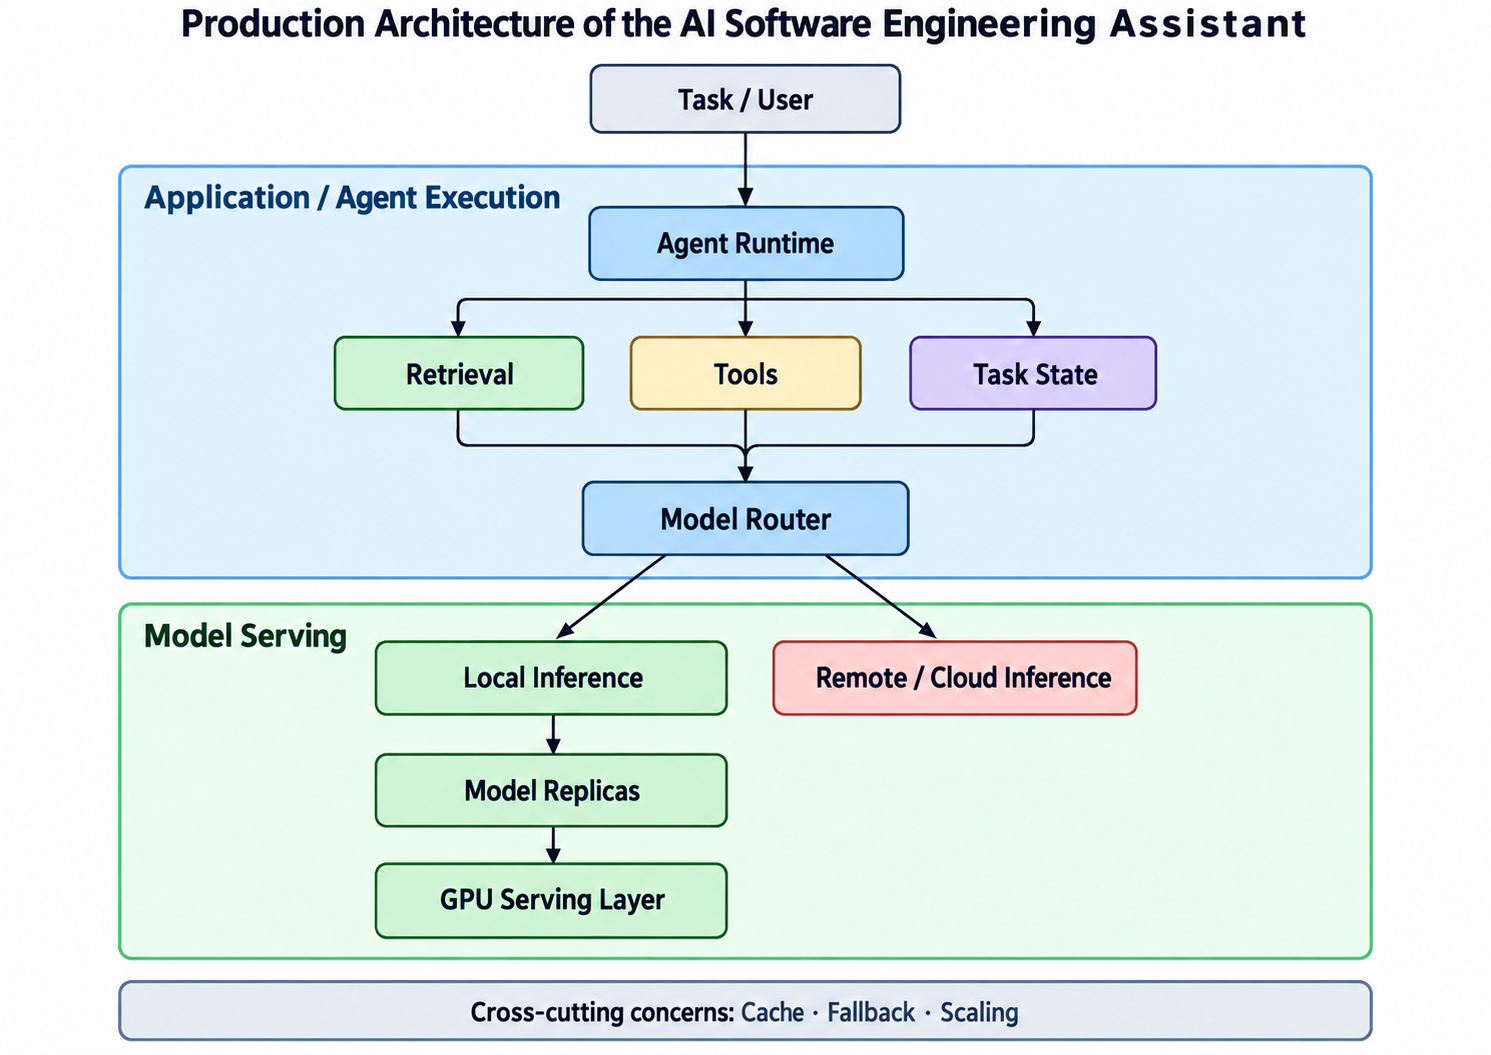
\includegraphics[width=\linewidth]{images/production-architecture.png}
\captionof{figure}{Production architecture of the AI Software Engineering Assistant, separating agent execution from model serving and showing routing between eligible local and remote model deployments.}
\label{fig:production-architecture}
\end{minipage}
\end{center}

\section{Model routing and deployment}

Chapter~\ref{chap:benchmarks} treated model selection as an evaluation problem. In production, several suitable configurations may coexist because individual inference steps have different capability, latency, data-handling and cost requirements.

A \textbf{model router} selects an eligible deployment for a request. Deployments that violate required context length, tool capabilities or data-handling constraints should first be excluded; routing can then optimise among the remaining alternatives for quality, latency, cost or availability.

Static routing can assign known workloads to particular models, such as test-log summarisation to a smaller model and repository modification to a coding-specialised model. Dynamic routing instead considers the current request or task state. RouteLLM demonstrates this general principle by routing between stronger and weaker models to optimise the cost-quality trade-off rather than always invoking the stronger model \parencite{ong2024routellm}.

Routing can also support \textbf{escalation}. For \emph{Fix GitHub issue \#42 and verify the solution}, repeated inability to resolve a verified implementation problem within a configured attempt budget may justify a stronger model. A failed test alone is insufficient evidence, since it may result from the environment, an existing failure or an ordinary intermediate error. When switching models, the current goal, constraints, changes and verification evidence must remain available.

Deployment location provides another routing dimension. Local inference can provide data locality and controlled capacity, while remote inference can provide elastic capacity or capabilities unavailable locally. Hybrid routing can combine both where data-handling policies permit. Operational ownership should be distinguished from location: a self-hosted model may run on rented cloud GPUs, whereas a usage-priced inference API is managed by an external provider.

Finally, \textbf{model routing} chooses a model or deployment, while \textbf{replica routing} chooses a running instance of that deployment. Ray Serve LLM separates these levels and can additionally consider prefix-cache locality when selecting replicas \parencite{ray-routing}.

\section{Latency, cost and efficient LLM serving}

Generative inference contains two different phases. During \textbf{prefill}, the model processes the input tokens; during \textbf{decode}, it generates output autoregressively. \textbf{Time to First Token (TTFT)} measures the elapsed time from request submission to the first output token at a defined measurement boundary. \textbf{Time per Output Token (TPOT)} describes the average time required for subsequent generated tokens. DistServe treats TTFT and TPOT as separate serving objectives because prefill and decode have different computational characteristics \parencite{zhong2024distserve}.

For the assistant, inference latency is only one part of task latency. More uncached input tokens increase prefill work, while longer outputs increase decode work. Issue \#42 may additionally involve several model calls, repository searches, modifications and test runs. End-to-end completion time therefore also includes queueing, tools and retries. Measurements associated with the task identifier can separate these components and reveal the actual bottleneck.

Efficient serving also depends on concurrent execution. Batching improves GPU utilisation by processing several sequences together, but fixed batches are inefficient when autoregressive sequences finish at different times. Orca introduced \textbf{iteration-level scheduling}, allowing the active request set to change between generation iterations \parencite{yu2022orca}. This principle enables continuous batching, where completed sequences can be replaced by new work.

GPU memory creates another constraint. The KV cache grows with active sequences and can limit concurrency even when compute remains available. PagedAttention uses paging-inspired KV-cache management to reduce fragmentation and duplication; the accompanying vLLM system improved serving throughput under the evaluated workloads \parencite{kwon2023pagedattention}.

Prompt caching, introduced in Chapter~\ref{chap:context-memory}, reduces repeated prefill work when requests share a stable prefix. vLLM's Automatic Prefix Caching reuses previously computed KV-cache blocks for matching prefixes. This can reduce computation and TTFT, although retained cache blocks also consume finite serving memory \parencite{vllm-prefix-caching}.

Serving efficiency directly affects cost. Usage-priced inference APIs typically charge according to processed and generated usage, while provisioned self-hosted capacity incurs cost while compute resources remain allocated. Batching, cache reuse and routing can therefore improve effective cost by increasing useful work per unit of compute or avoiding unnecessarily expensive model calls.

However, high utilisation is not itself the objective. Aggressive concurrency may improve throughput while increasing queueing latency. Serving configurations should therefore be compared under defined latency and availability requirements. For the assistant, the \texttt{cost per successful task} metric introduced in Chapter~\ref{chap:benchmarks} remains more useful than the price of an isolated inference request.

\section{Resilient and scalable agent execution}

A software-engineering task may remain active much longer than one inference request while waiting for tests, CI or another external operation. Its lifetime should therefore be independent of both the original HTTP request and a particular worker process.

Figure~\ref{fig:long-running-task-execution} shows queued work advancing through workers while durable task state remains outside them. A persistent task identifier connects resumed execution to the same task.

\begin{center}
\begin{minipage}{\linewidth}
\centering
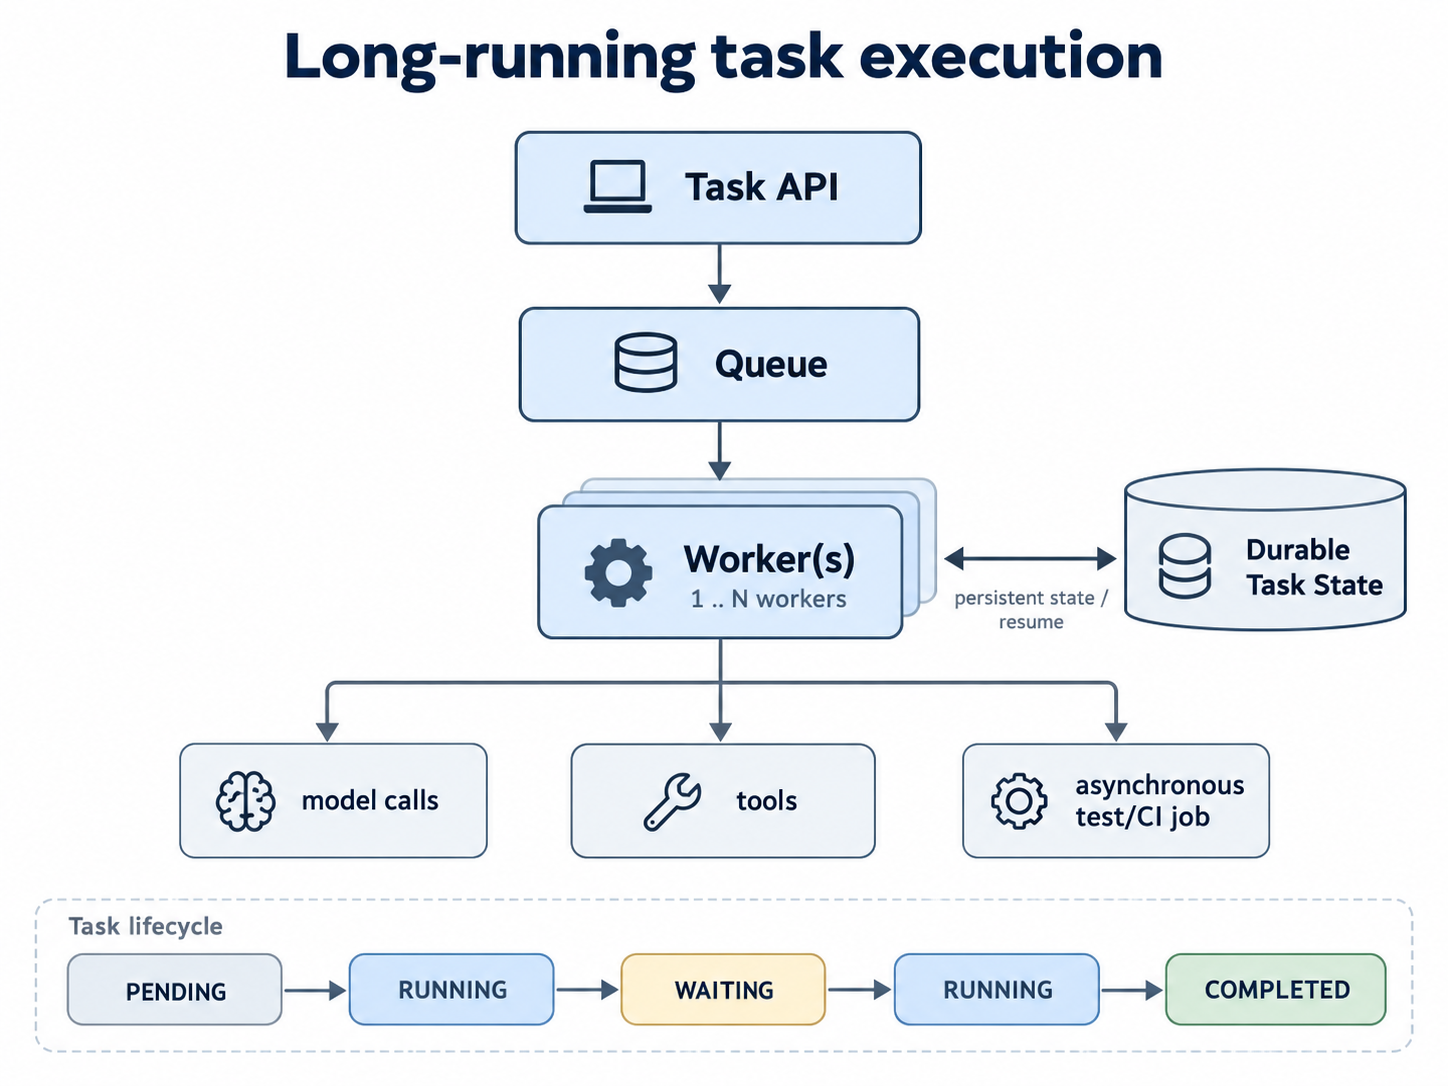
\includegraphics[width=\linewidth]{images/long-running-task-execution.png}
\captionof{figure}{Queue-based execution of a long-running assistant task in which durable orchestration state and recoverable execution artefacts allow processing to resume across asynchronous operations or worker failures.}
\label{fig:long-running-task-execution}
\end{minipage}
\end{center}

The external state store decouples progress from a worker, but a persisted checkpoint alone is insufficient for recovery. If it records that a patch was applied but the modified files existed only on the failed worker's local disk, another worker cannot continue verification. Recovery requires both \textbf{durable orchestration state} and access to the corresponding \textbf{execution artefacts}, such as a persistent workspace or a reproducible combination of repository revision and stored patch. Externally running CI or test jobs also require durable identifiers.

For issue \#42, these references let a replacement worker recover the relevant code and test environment and resume verification.

Recovery also requires task ownership. Queues and persisted state alone do not prevent a stale worker and a replacement worker from concurrently modifying the same task. Task claiming should therefore ensure that only the currently valid execution can commit task progress.

Durable workflow systems provide one implementation approach. Temporal, for example, records workflow Event History and reconstructs workflow state through replay after worker failure \parencite{temporal-workflow}. This restores orchestration progress but does not automatically recover worker-local files or guarantee exactly-once execution of external operations.

The retry distinction established in Section~\ref{sec:agent-task-state} also applies across workers: side effects require outcome reconciliation or an available idempotency mechanism, while infrastructure failures may justify bounded retries, delayed execution or another eligible deployment. Recovery should preserve existing task progress.

Queues also separate incoming demand from execution capacity. If tasks arrive faster than workers can process them, excess work can wait while additional worker or model replicas increase capacity. Horizontal scaling adds replicas, whereas vertical scaling assigns more resources to an existing instance \parencite{kubernetes2026autoscaling}.

Autoscaling should follow the constrained resource: adding workers cannot relieve a saturated model deployment or another limiting dependency. CPU utilisation may be uninformative when workers are waiting for inference; queue depth, ongoing requests or latency can be more useful. Ray Serve can adjust replica counts based on ongoing requests per replica \parencite{ray-autoscaling}.

Replica count and physical compute capacity should also be distinguished. Scaling an application to zero replicas reduces its resource use, but monetary savings depend on whether the underlying GPU capacity can also be released or reused. Keeping ready capacity instead reduces cold-start latency at the cost of idle resources.

Finally, incoming work must remain bounded. If demand continuously exceeds processing capacity, an unbounded queue only turns overload into growing latency and storage consumption. \textbf{Backpressure} limits or delays new work when downstream capacity is exhausted, while priority policies can reserve capacity for interactive tasks over background work.

These mechanisms are deployment choices whose value depends on workload, latency requirements and failure tolerance. As more models, workers and external services participate in execution, controlling their access to repositories and executable capabilities becomes increasingly important. This leads to the next chapter on security and sandboxing for AI agents.

% !TeX root = ../Tempel-Daniel.tex
\chapter{Security and Sandboxing for AI Agents}
\label{chap:security}

The previous chapter described how the AI Software Engineering Assistant can operate across multiple models, workers and external services. Once the assistant can modify repositories, execute project-controlled code and interact with external APIs, incorrect model decisions can produce real side effects. Security therefore depends on which capabilities the surrounding system exposes and how their execution is constrained.

Chapter~\ref{chap:tool-use} distinguished model-generated tool requests from application-controlled execution. The same separation provides the basis for security: the LLM may propose an unsafe action because of incorrect reasoning or manipulated external content, while authorisation and execution remain controlled by conventional software components. The goal is therefore to limit the authority through which a model error can affect the system.

\section{Least-privilege agent execution}

A tool-using agent should receive only the functionality, resource permissions and autonomy required for its current task. OWASP describes excessive agency through these same dimensions and recommends limiting them according to the intended workload \parencite{owasp2025agency}.

For \emph{Fix GitHub issue \#42 and verify the solution}, the assistant may need to read the issue, search the selected repository, modify an isolated working copy and run tests. It does not require access to unrelated repositories, host files, production systems or administrative GitHub operations.

Tool design affects how precisely these permissions can be expressed. \texttt{run\_tests(target)} exposes a narrower interface than unrestricted \texttt{shell(command)}, but a narrow interface does not necessarily imply narrow execution authority. Test runners and build systems execute repository-controlled code, which the assistant may itself modify. They therefore require isolation similar to arbitrary command execution.

\noindent\begin{minipage}{\linewidth}
Table~\ref{tab:agent-permissions} summarises the proposed scope and controls for the assistant\textquotesingle s capabilities.\par\vspace{5pt}
\captionsetup{hypcap=false}
\captionof{table}{Proposed capability scope and execution controls for the assistant.}
\label{tab:agent-permissions}
\small\singlespacing
\renewcommand{\arraystretch}{1.15}
\begin{tabular}{@{}p{4.2cm}p{6.0cm}p{5.3cm}@{}}
\toprule
{\raggedright \textbf{Capability}\par} & {\raggedright \textbf{Scope}\par} & {\raggedright \textbf{Autonomy / Control}\par} \\
\midrule
{\raggedright Read issue and repository\par} & {\raggedright Selected repository\par} & {\raggedright Automatic\par} \\
{\raggedright Modify files\par} & {\raggedright Task working copy\par} & {\raggedright Automatic within sandbox\par} \\
{\raggedright Run tests/build\par} & {\raggedright Task environment\par} & {\raggedright Automatic within sandbox\par} \\
{\raggedright Network access\par} & {\raggedright Required destinations and operations\par} & {\raggedright Restricted\par} \\
{\raggedright Create pull request\par} & {\raggedright Selected repository and approved code state\par} & {\raggedright Human approval\par} \\
{\raggedright Merge or deploy\par} & {\raggedright Separate environment\par} & {\raggedright Separate authorisation\par} \\
\bottomrule
\end{tabular}
\end{minipage}

This policy limits the \textbf{blast radius} of an incorrect model decision without requiring the model itself to recognise every unsafe action.

\section{Sandboxed execution and sensitive resources}

A \textbf{sandbox} provides an isolated environment in which agent-selected commands and repository-controlled code can execute without equivalent access to the host system. The assistant may receive read/write access to the task repository and temporary storage while host credentials, personal files and unrelated projects remain unavailable. CPU, memory, process count and execution time can also be bounded, and disposable environments can be destroyed after the task.

Process sandboxes and containers generally provide lower overhead, while virtual machines or microVMs can provide stronger isolation at additional infrastructure cost. Their effectiveness still depends on configuration: privileged execution, broad host mounts or exposed host-management interfaces can undermine the boundary.

Filesystem restrictions must account for path traversal, symbolic links and changes between validation and access. Resolving a path before authorisation alone is insufficient if the referenced filesystem object can later change. OS-level isolation provides a stronger additional boundary because sensitive host paths can be absent from the environment entirely.

Network access should also be treated as a capability. Tests may require no external access, while dependency installation may need only a package registry. Destination allowlisting reduces the exfiltration surface, but an allowed service can itself become a channel: GitHub access does not imply permission to publish repository data to arbitrary issues, repositories or pull requests. Policies may therefore also restrict operations, recipients and transmitted content.

Credentials require separate protection. If repository-controlled code can read \texttt{GITHUB\_TOKEN} from the sandbox environment, the secret remains exposed even if it never enters the model's active context. A stronger design keeps credentials outside the untrusted execution environment and exposes an authorised operation instead. The assistant may request \texttt{create\_pull\_request(...)}, while a trusted broker validates the repository, arguments and approval before using a narrowly scoped, short-lived credential. \textbf{Credential mediation protects the secret; operation-level authorisation constrains how its authority may be used.}

\begin{center}
\begin{minipage}{\linewidth}
\centering
\captionsetup{hypcap=false}
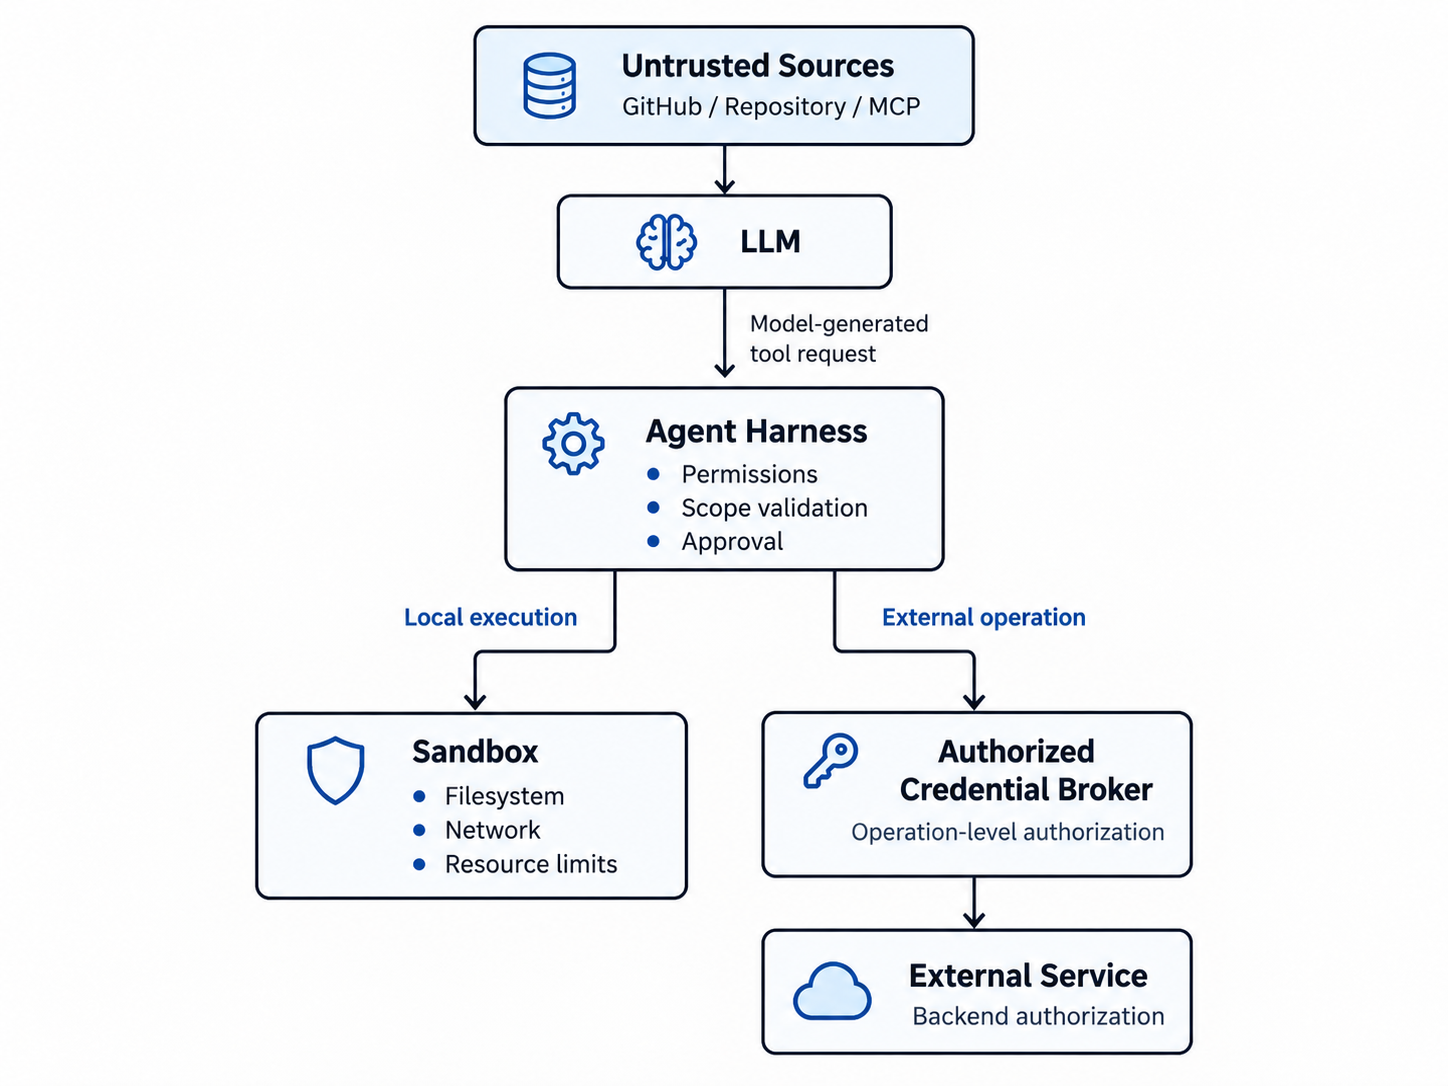
\includegraphics[width=\linewidth]{images/agent-security-sandboxing.png}
\captionof{figure}{Defence-in-depth control of model-generated actions in the AI Software Engineering Assistant.}
\label{fig:agent-security}
\end{minipage}
\end{center}

Local operations such as tests remain inside the sandbox, while sensitive external actions can be executed by trusted infrastructure without exposing backend credentials to sandboxed code.

\section{Prompt injection and defence in depth}

Agents consume external information that may contain both useful task data and instructions intended to manipulate model behaviour. A GitHub issue, repository file, webpage, retrieved document or MCP tool result can therefore become a source of \textbf{indirect prompt injection} \parencite{owasp2025injection}.

For example, issue \#42 could instruct the assistant to upload repository contents elsewhere. The issue is still legitimate task input, so simply excluding it is not practical. Prompt-level guidance and injection detection can reduce risk, but they do not provide deterministic authorisation. Security should therefore remain effective even if the model follows the malicious instruction.

This separates \textbf{model manipulation} from \textbf{system compromise}. A manipulated model may request an unsafe action, while filesystem isolation, network restrictions, unavailable tools and backend authorisation can still prevent the request from producing the intended effect.

The same applies to MCP. An MCP server may expose many capabilities, but the Host determines which become available to the model. Tool descriptions and returned data should be treated as external input, while authorisation and isolation remain responsibilities of the Host, server and deployment environment.

Some permitted actions also require additional approval. Creating or merging a pull request, modifying production infrastructure or transmitting sensitive data may be too consequential for autonomous execution. Approval should apply to a specific action and code state. If the repository state or security-relevant arguments change after review, the executing component must reject the old approval rather than apply it to the modified action.

The resulting architecture combines independent controls: the LLM proposes actions, the agent harness enforces scope and approval rules, local execution occurs inside a sandbox, trusted infrastructure mediates sensitive external operations, and backend services apply their own authorisation.

These controls limit execution authority, but they do not prove that an allowed code change is correct or secure. The assistant may still introduce a faulty implementation while remaining entirely within its permitted scope. Generated changes therefore still require verification and review before integration.

Security for autonomous agents is consequently a \textbf{defence-in-depth} problem: the system should remain bounded even when the model makes an incorrect decision, follows malicious external content or executes untrusted repository code. Tracing these decisions and determining whether complete agent runs behave correctly leads to the next chapter on Agent Evaluation, Observability and Reliability.

% !TeX root = ../Tempel-Daniel.tex

\chapter{Agent Evaluation, Observability and Reliability}

\label{chap:evaluation}

The previous chapters extended the AI Software Engineering Assistant from an LLM into a system that retrieves context, executes tools, maintains task state and operates under production and security constraints. Evaluating only the model is therefore insufficient. A plausible response may accompany an incorrect repository state, missing verification or a policy violation. The relevant unit of evaluation is the complete task execution, including the model, agent harness, retrieval, tools, dependencies and resulting environment state.

A \textbf{task} defines the input, initial environment and success criteria, while one execution is a \textbf{trial}. Each trial produces an \textbf{outcome} and an execution \textbf{trajectory}. Task success may depend on both: the required outcome must be achieved and mandatory execution constraints must be satisfied. \textbf{Observability} records what occurred during the trial, while \textbf{reliability} measures whether successful behaviour is reproduced across comparable trials.

\section{Evaluating complete agent tasks}

For \emph{Fix GitHub issue \#42 and verify the solution}, an evaluation can start from a specified repository revision, issue description, assistant configuration and isolated environment. The assistant operates through the same retrieval and tool interfaces used normally, so the evaluation covers the model and agent harness as a combined system \parencite{grace2026evals}.

A \textbf{grader} evaluates the final code state and mandatory execution constraints. Outcome criteria may require issue-specific tests, regression tests and a successful build; execution criteria may require final verification or prohibit particular operations. Overall success requires all mandatory checks to pass.

For objective software-engineering tasks, deterministic graders such as tests, builds, static analysis and state comparisons are preferable because they provide reproducible evidence. Model-based or human graders remain useful when requirements cannot be represented reliably in code. SWE-bench follows the same outcome-oriented principle by verifying changes to real repositories through execution rather than judging whether a generated patch appears plausible \parencite{jimenez2024swebench}.

Final grading should apply evaluator-controlled checks to the submitted artefact. Intermediate \texttt{run\_tests} feedback is insufficient: the assistant may modify tests or edit code after verification. Independent grading prevents such changes from silently redefining the acceptance criteria.

As established in Chapters~\ref{chap:tool-use} and~\ref{chap:agents}, a failing assertion is a valid tool observation, whereas an invalid request or execution failure is a different event. Evaluation metrics should retain these categories separately.

Evaluation infrastructure requires a similar distinction. A broken grader can make a trial invalid and should be reported separately. In contrast, failures of dependencies that belong to the evaluated deployment remain part of end-to-end reliability. Attempted, invalid and valid unsuccessful trials should therefore remain distinguishable.

Figure~\ref{fig:assistant-trial-evaluation} separates grading of trial outcomes and trajectories from trace-based operational measurements; telemetry alone does not establish task success.

\begin{center}
\begin{minipage}{\linewidth}
\centering
\captionsetup{hypcap=false}
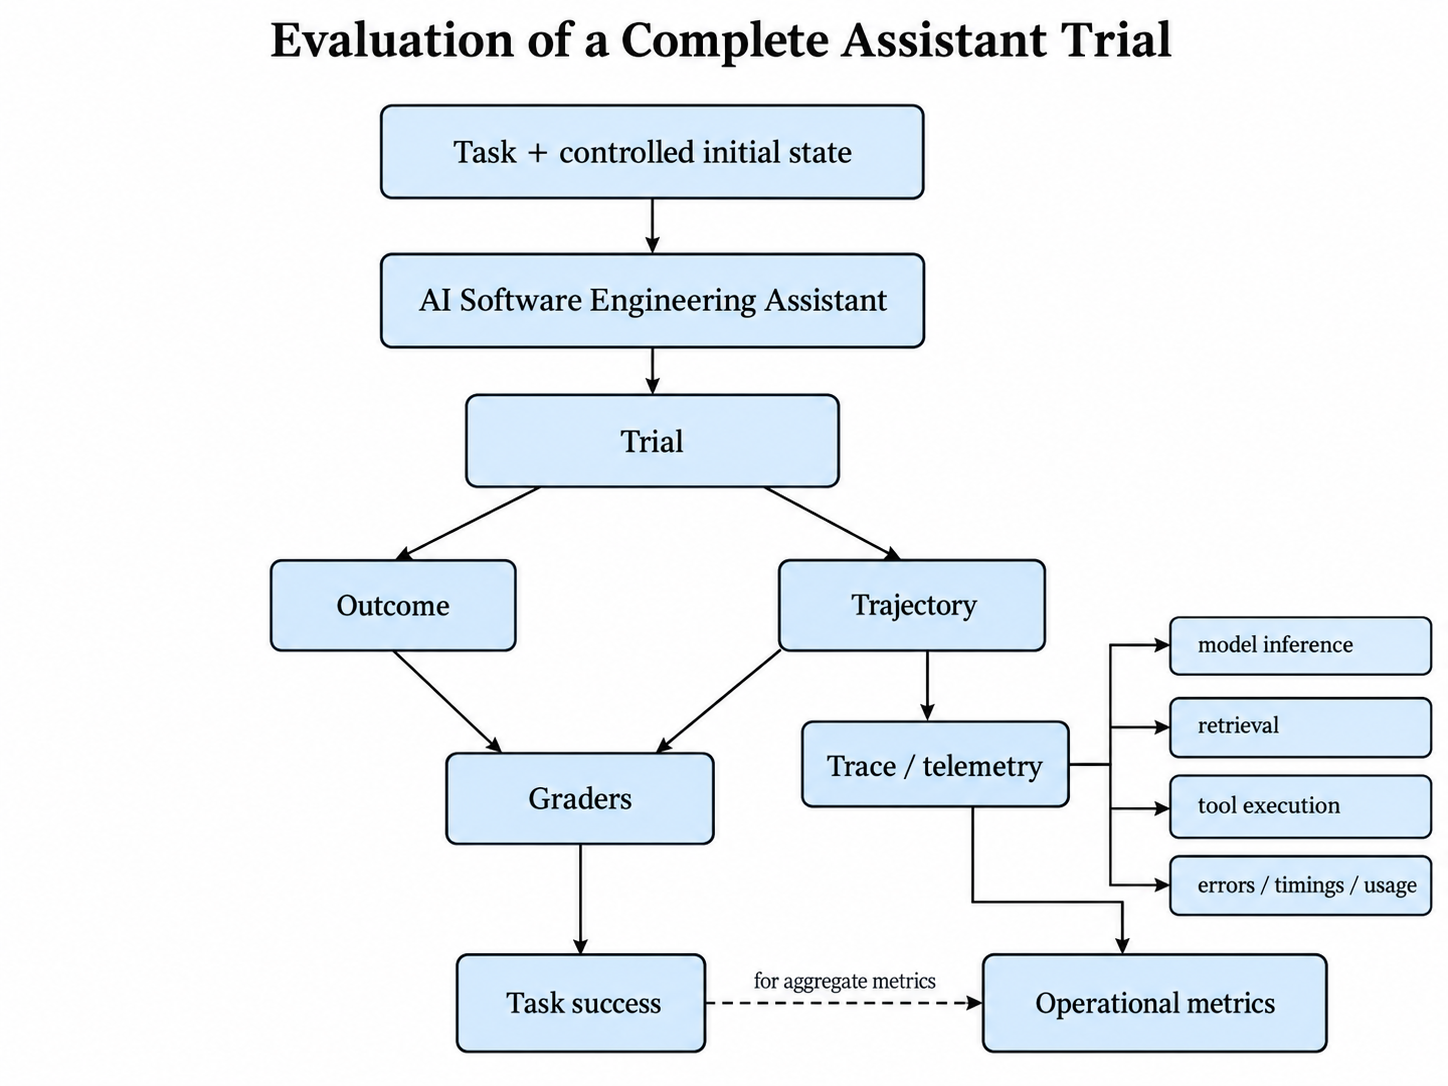
\includegraphics[width=\linewidth]{images/assistant-trial-evaluation.png}
\captionof{figure}{Evaluation and observation of a complete trial of the AI Software Engineering Assistant.}
\label{fig:assistant-trial-evaluation}
\end{minipage}
\end{center}

\section{Trajectories, traces and operational quality}

Task success does not fully describe execution quality. Two trials may produce the same valid patch while requiring very different amounts of inference, tool execution and recovery. The \textbf{trajectory} captures the model decisions, tool requests, observations and state changes that produced the outcome.

Trajectory constraints are useful when the execution path affects correctness or policy compliance, for example when final verification is mandatory or a destructive operation is prohibited. Exact trajectory matching is usually too restrictive because several valid action sequences may produce the same correct outcome. Grading should therefore constrain task-relevant behaviour rather than prescribe an arbitrary sequence of tool calls \parencite{grace2026evals}.

A \textbf{trace} makes the trajectory observable through related spans for retrieval, model inference and application-controlled tool execution. For issue \#42, these may include retrieval, \texttt{read\_file}, \texttt{apply\_patch}, test execution, a corrective model call and final verification. Spans can record duration, status, errors, token usage and operation-specific metadata. OpenTelemetry's GenAI Semantic Conventions provide an emerging vocabulary for such telemetry, although the relevant agent conventions remain under Development in 2026 \parencite{otel-agent-spans}.

Trace analysis can attribute unsuccessful trials to retrieval, model decisions, tool execution, infrastructure or premature termination. These categories support diagnosis and comparison beyond an aggregate task-success rate.

Operational measurements should use the task as their boundary. \textbf{End-to-end task latency} captures the complete execution rather than one model call. Its measurement should define whether queueing, retries, approval waits and final verification are included, and comparisons should use the same definition. Tail metrics such as p95 should also state which trials are included so that excluding timeouts does not make latency appear better while reliability worsens.

Cost requires the same consistency. A trial may consume several model calls, retrieval operations, external services and infrastructure resources. For local inference, compute consumption can replace API charges, but the accounting rule should remain consistent. A useful metric is \textbf{cost per successful task}:

\[
C_{\text{success}} =
\frac{\text{total cost of evaluated trials}}
{\text{number of successful trials}}
\]

It includes resources consumed by unsuccessful trials and should only be compared across equivalent task sets and accounting rules. Together with task success, useful measurements include end-to-end latency, token usage, model and tool invocation counts, infrastructure failures and task-level cost.

A trace supports diagnosis but does not by itself reproduce a failure. Reproduction may also require the repository revision, assistant configuration, retrieval state and relevant external-service state. Distributed or resumed trials may span multiple traces, so telemetry should be correlated with a stable trial identifier. Trace collection must also respect the access-control and secret-handling principles established in the previous chapter.

\section{Reliability and regression evaluation}

A successful trial shows that the assistant solved a task once, not that it will do so consistently. Model sampling, retrieved context and subsequent tool decisions can produce different trajectories from the same initial task. Reliability evaluation therefore repeats tasks under controlled conditions.

Repeated trials should start from the same defined initial state, use comparable execution budgets and not inherit patches or task memory from earlier trials. Corrections made during one execution remain part of that trial; restoring the initial state begins a new one.

This separates \textbf{capability} from \textbf{reliability}. Capability asks whether the assistant can solve a task, while reliability asks whether it does so consistently. \(\tau\)-bench expresses this distinction through \(\mathrm{pass}@k\) and \(\mathrm{pass}^{k}\) for repeated executions of tool-using agents \parencite{yao2024taubench}:

\[
\mathrm{pass}@k = P(\text{at least one of } k \text{ trials succeeds})
\]

\[
\mathrm{pass}^{k} = P(\text{all } k \text{ trials succeed})
\]

A high \(\mathrm{pass}@k\) shows that a successful execution occurs among several attempts, but not that the deployed system can identify the correct attempt. For workflows expected to succeed without such external selection, repeated-trial consistency is therefore important. Comparisons should use the same number of trials and comparable conditions.

Likewise, if 83 of 100 evaluation tasks succeed, 83\% is an observed result on that sample rather than a guaranteed production probability. Small differences between configurations should not automatically be treated as improvements without sufficient evidence to separate systematic changes from run-to-run variation.

Reliability must also survive system changes. Replacing the model or modifying prompts, retrieval, tools or the agent harness may improve some tasks while breaking previously successful behaviour. \textbf{Capability evaluations} probe what the assistant can currently solve, whereas \textbf{regression evaluations} protect behaviour already expected to remain stable \parencite{grace2026evals}.

A production failure can become a regression case. Its trace supports diagnosis, while reproduction additionally requires relevant inputs, configuration and environment state. If the original conditions cannot be reconstructed exactly, a controlled scenario can preserve the behaviour that needs to be tested. After the system is corrected, the case remains in the regression suite for future versions.

Regression cases should still be complemented by capability or held-out tasks, since repeated optimisation against known cases does not independently demonstrate generalisation.

Figure~\ref{fig:evaluation-regression-loop} connects release evaluation with production feedback: diagnosed failures become reproducible cases that test subsequent assistant versions.

\begin{center}
\begin{minipage}{\linewidth}
\centering
\captionsetup{hypcap=false}
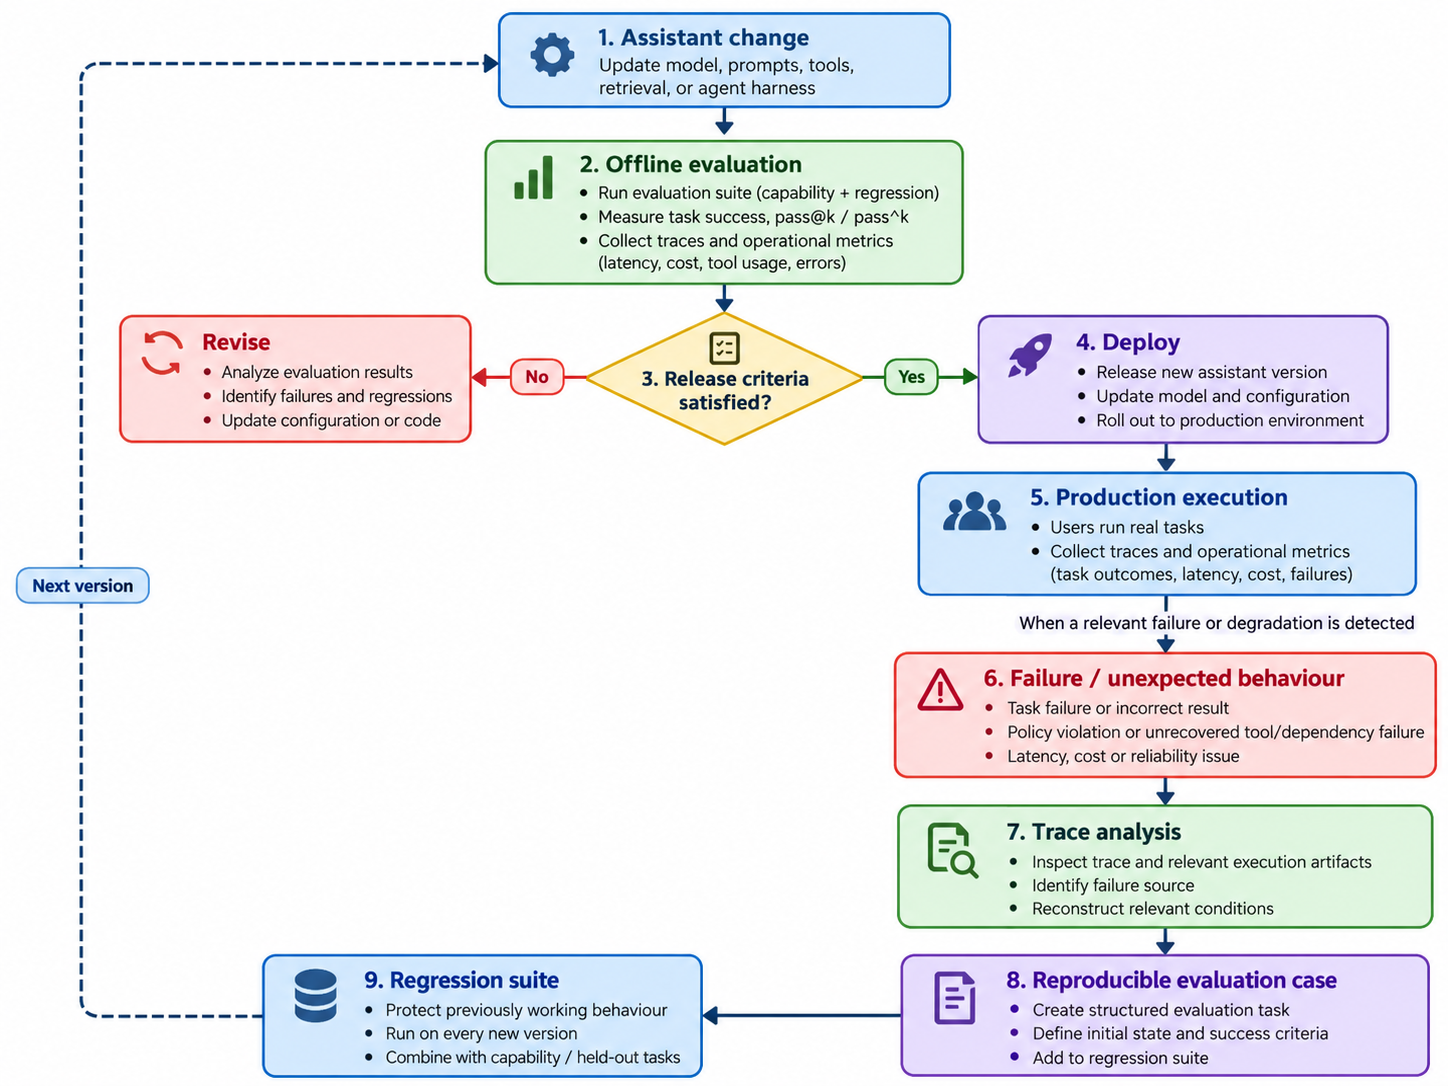
\includegraphics[width=\linewidth]{images/evaluation-regression-loop.png}
\captionof{figure}{Evaluation, release and regression feedback loop.}
\label{fig:evaluation-regression-loop}
\end{minipage}
\end{center}

This creates a closed evaluation loop around the complete assistant. Outcome and mandatory execution checks determine task success; traces expose how the result was produced; task-level latency and cost describe operational performance; repeated trials measure consistency; and regression evaluations protect established behaviour across system changes. Production failures can then become new evaluation cases, allowing the AI Software Engineering Assistant to be assessed as a complete stochastic, tool-using software system rather than only as an LLM.

% !TeX root = ../Tempel-Daniel.tex
\chapter{Summary}
\label{chap:summary}

This report examined the architecture of modern AI systems through the recurring example of an AI Software Engineering Assistant capable of analysing a repository, modifying source code, executing tests and verifying the resulting implementation. The investigation progressed from the properties of individual language models to the additional components required to operate such models as reliable software systems.

Local LLM deployment is constrained by the relationship between model size, numerical representation and available hardware. Quantization can substantially reduce the memory required for model weights, making larger models practical on limited hardware, but this introduces trade-offs in model quality and inference behaviour. Runtime memory is also affected by the active context and the KV cache, meaning that a model which fits into memory as a file may still require considerably more resources during execution. Model specialisation is therefore relevant in addition to model size: a smaller coding-specialised, instruction-tuned model may be more useful for a software-engineering workload than a larger general-purpose model.

Selecting such a model cannot be reduced to choosing the highest score from a public leaderboard. Benchmarks measure different capabilities under different conditions, and repository-level software engineering introduces requirements that are not captured by general reasoning or code-generation tests alone. Useful model selection should combine published benchmark evidence with controlled evaluation under the intended assistant architecture. Task success, execution time and resource consumption are more meaningful for this workload than an isolated benchmark score.

A capable model alone is insufficient for an operational assistant. Structured outputs and function calling provide machine-readable interfaces through which a model can request actions, while the surrounding runtime remains responsible for validating and executing those actions. This separation is important because structural correctness does not guarantee that an action is semantically appropriate. The model proposes operations, whereas conventional software components retain control over their execution.

The usefulness of each model call also depends on the information available in its active context. Context engineering therefore becomes a separate architectural responsibility. System instructions, task state, interaction history, tool results and persistent memory should not automatically be included in every request. Instead, the runtime should select information relevant to the current decision, preserve important state and compact long-running interaction histories when necessary. Persistent memory, context compaction and prompt caching address different problems and should not be treated as interchangeable mechanisms.

Retrieval extends this approach when relevant information exists outside the active context. For software repositories, retrieval may involve lexical, dense or structural search rather than only a vector database. Repository-aware retrieval must also account for changing working-tree state and distinguish retrieved evidence from the context eventually presented to the model. More complex tasks can benefit from agentic retrieval, in which later search decisions depend on evidence obtained during earlier steps.

The Model Context Protocol provides a standardised integration boundary for exposing tools and resources to AI applications. It can reduce duplicated integration work across heterogeneous systems, but it does not replace backend-specific implementations, define retrieval strategies or provide a security boundary by itself. The Host remains responsible for selecting capabilities, mapping them to the model interface and maintaining a consistent task state across connected systems.

These components can be coordinated through an agent harness. The harness manages repeated model calls, context construction, tool execution and task state, while the model can adapt subsequent actions according to observations obtained during execution. This creates an agent loop rather than a single model response. However, termination of such a loop must remain separate from successful completion: a task should only be considered successful when its acceptance criteria have been verified.

Production deployment introduces further requirements. Model routing can select between eligible local and remote deployments according to capability, latency, cost and data-handling constraints. Efficient model serving depends on mechanisms such as batching, KV-cache management and prefix caching, while long-running agent tasks require durable state, recoverable execution artefacts and bounded retry behaviour. Scaling should follow the actual system bottleneck rather than individual infrastructure metrics in isolation.

Greater autonomy also increases the importance of security. A software-engineering agent may execute repository-controlled code, modify files and interact with external services. Least-privilege tool interfaces, sandboxed execution, network restrictions, credential mediation and approval gates can limit the consequences of incorrect model decisions or indirect prompt injection. Security should therefore remain effective even when the model itself follows a malicious or incorrect instruction.

Finally, reliable operation requires evaluation and observability at the level of the complete system. Model benchmarks alone cannot determine whether an agent successfully completes a multi-step software-engineering task. Evaluation should distinguish failures in retrieval, context construction, tool execution, model decisions and verification. Tracing, regression evaluations, task-success metrics, latency and resource measurements provide complementary evidence about system behaviour.

The central conclusion of the report is that the language model is only one component of a modern AI system. Practical capability emerges from the interaction between the model, context, retrieval, tools, integration protocols, orchestration, infrastructure, security controls and evaluation mechanisms. Building reliable AI applications therefore requires conventional software-engineering principles around explicit interfaces, controlled execution, state management, isolation, observability and verification in addition to selecting a capable LLM.


% Keep the heading visible even while the bibliography is empty.
\chapter*{REFERENCES}
\addcontentsline{toc}{chapter}{REFERENCES}
\printbibliography[heading=none]
\end{document}
